\documentclass[a4paper,openany]{book}

%#############################################################################
% Paquetes utilizados
\usepackage[utf8]{inputenc} % codigo 
\usepackage[spanish]{babel} % español
\usepackage{graphicx} % insertar imagenes
\usepackage[table, xcdraw]{xcolor} % color
\usepackage[most]{tcolorbox} % cuadros https://es.overleaf.com/latex/examples/drawing-coloured-boxes-using-tcolorbox/pvknncpjyfbp
\usepackage[left=2.54cm, right=2.54cm, top=2.54cm,bottom=2.54cm ]{geometry} % texwidth tendra un margen de 2cm derecha izquierda
\usepackage{fancyhdr} % estilo de la pag
\usepackage[hidelinks]{hyperref} % Hipervinculos
\usepackage{parskip} % Quita la salgria y pone un espacio en blanco
\usepackage{smartdiagram} % Insertar diagramas
\usepackage{listings} % Insertar codigo en el documento
\usepackage{zed-csp} % insertar tablas
\usepackage{wrapfig} %preámbulo
\usepackage{setspace}
\usepackage{pgfgantt}
\usepackage{minted} %insertar codigo coloreado
\usepackage{color, colortbl}
\usepackage{url}
\usepackage{pdfpages}
\usepackage{pdflscape} %poner pdf horizontal
\usepackage[square,numbers]{natbib}
\usepackage{tikz}
\usepackage{datetime}

%#######################################################################
%Cronograma
\definecolor{barblue}{RGB}{153,204,254}
\definecolor{groupblue}{RGB}{51,102,254}
\definecolor{linkred}{RGB}{165,0,33}
\sffamily

%#############################################################################
% Info del documento
\title{Trabajo Final}
\author{Blanco Emanuel .A}

%#############################################################################
% Colores
% Definición de colores usados en la portada
\definecolor{epsc:oscuro}{HTML}{0063ae}
\definecolor{epsc:medio}{HTML}{4C5CC5}
\definecolor{epsc:verde}{HTML}{009cb5}
\definecolor{epsc:claro}{HTML}{3FCFD5}
\definecolor{PORTADA_0}{cmyk}{1.00,0.00,0.07,0.28,1.00}
\definecolor{PORTADA_1}{cmyk}{0.58,0.55,0.00,0.44,1.00}
\definecolor{friendlyGray}{HTML}{f0f0f0}
\definecolor{azPortada}{HTML}{A52FFC}
\definecolor{vePortada}{HTML}{0DF3B1}
\definecolor{roPortada}{HTML}{EC40A5}
\definecolor{nePortada}{HTML}{070308}

\renewcommand{\lstlistingname}{Código} % cambiar el caption del codigo
\definecolor{codegreen}{rgb}{0,0.6,0}
\definecolor{codegray}{rgb}{0.5,0.5,0.5}
\definecolor{codepurple}{rgb}{0.58,0,0.82}
\definecolor{backcolour}{rgb}{0.95,0.95,0.92}

\lstdefinestyle{mystyle}{ % Color de sintaxis https://es.overleaf.com/learn/latex/Code_listing
    backgroundcolor=\color{backcolour},   
    commentstyle=\color{codegreen},
    keywordstyle=\color{magenta},
    numberstyle=\tiny\color{codegray},
    stringstyle=\color{codepurple},
    basicstyle=\ttfamily\footnotesize,
    breakatwhitespace=false,         
    breaklines=true,                 
    captionpos=b,                    
    keepspaces=true,                 
    numbers=left,                    
    numbersep=5pt,                  
    showspaces=false,                
    showstringspaces=false,
    showtabs=false,                  
    tabsize=2
}

\lstset{style=mystyle}

%#############################################################################
% variables
\newcommand{\logoPortada}{imagenes/portada/portada.jpg}
\newcommand{\logoFich}{imagenes/portada/fich.jpg}
\newcommand{\logoUnl}{imagenes/portada/portada.jpg}
\newcommand{\nameAuthor}{Blanco Emanuel A.}
\newcommand{\startdate}{26 de Junio 2022}
\newdateformat{monthyeardate}{\monthname, \THEYEAR}

%#############################################################################
% Comienzo del documento

\begin{document}
    
    \cfoot{\thepage} % Numero de pag
    
    \frontmatter

	
\thispagestyle{empty}

\begin{tikzpicture}[remember picture, overlay]
	% Top
	\node [anchor=north east, inner sep=0pt]  at (current page.north east)%
	{
\includegraphics[height=6cm]{imagenes/Portada/arriba.png}};
	% Bottom
	\node [anchor=south west, inner sep=0pt]  at (current page.south west)%
	{
\includegraphics[height=6cm]{imagenes/Portada/abajo.jpg}};
	\node (uco) [anchor=south east, inner sep=0pt, xshift=-10mm, yshift=10mm]  at (current page.south east)%
	{
\includegraphics[height=6cm]{imagenes/Portada/unl_escudo.pdf}};
	\node [anchor=south east, inner sep=0pt, xshift=-10mm]  at (uco.south west)%	
	{
\includegraphics[height=6cm]{imagenes/Portada/fich.pdf}};
	
\end{tikzpicture}

% Título del trabajo, autor y directores
	{\color{epsc:oscuro}
	\centering                                                              

        {\LARGE\textbf{UNIVERISDAD NACIONAL DEL LITORAL}}\par\vspace{0.5cm}      

		{\large\textbf{FACULTAD DE INGENIERIA Y CIENCIAS HÍDRICAS}}\par        

	}

\begin{flushright}                                  
	
	{\color{epsc:verde} \rule{7cm}{0.5mm}}
	
\end{flushright}

\begin{center}
	
	\vspace*{2cm}
	
	
\includegraphics[width=12.5cm]{imagenes/Portada/fich_logo.png}
	
	\vspace{1cm}
	
	{\color{epsc:oscuro}
		
		\Large\textbf{TRABAJO FINAL}\par	
		
		\vspace{0.2cm}
		
		\textbf{MIGRACIÓN DE SOFTWARE PRIVATIVO A SOFTWARE LIBRE}
		
		\vspace{0.2cm}
		
	} \vspace{2mm}
	
	{\color{epsc:oscuro}
		
		{\itshape{baruja shen adonai elohim}}\vspace{1cm}
		
		{\color{epsc:verde}\rule[2cm]{7cm}{0.3mm}}
		
		\begin{center}
	
			{\large\textbf{Blanco Emanuel A.}}\par
			{\large\textbf{Universidad Nacional Del Litoral.}}\par
			{\large\textbf{Facultad de Ingeniería y Ciencias Hídricas.}} \par
			{\large\textbf{Tecnicatura Universitaria en Software Libre.}}\par
			{\large\textbf{Creative Commons Atribución-CompartirDerivadasIgual 2.5 (Argentina)}}
				
		\end{center}
		
		\vspace{0.7cm}
	
		\textbf{\monthyeardate{\today}}        % Fecha de compilación en formato mes, año
		
	}

\end{center}

\endinput
% la version de pdf del logo de la unles muy nueva para latex, compilar version mas vieja
%a) Convierte el archivo unl_escudo.pdf a una versión compatible: Utiliza una herramienta de conversión, como Ghostscript o Adobe Acrobat, para convertir el archivo unl_escudo.pdf a una versión anterior del formato PDF, como la versión 1.5. Asegúrate de guardar el archivo convertido en una ubicación accesible y actualiza la referencia en tu archivo LaTeX para apuntar al nuevo archivo convertido.
	
    \tableofcontents

    \mainmatter

    
\chapter{Introducción}\label{ch:ntroducción}


	Este trabajo es el resultado de un largo periodo formativo, el cual 
	concluyó en Diciembre del 2020. Lo desarrollado en esta página pretende 
	cumplir con los requisitos del Trabajo Final de la Tecnicatura Universitaria 
	en Software Libre.\par
	
	El trabajo desarrollado tuvo lugar en la sala de informática perteneciente 
	a la UNL, ubicada en el instituto de detención penal Nº 2 “Las Flores”. 
	El propósito de esta sala informática es posibilitar el acceso a personas 
	privadas de su libertad a distintas trayectorias educativas/culturales/laborales, 
	mediante el estudio a distancia a través de internet.\par
	
	El siguiente texto describe la migración de Software Propietario a Software Libre 
	realizada en el Aula Virtual de la UNL, en el penal de las flores.\par
	
	Los objetivos propuestos y a concretar fueron los siguientes:\par
	
	\begin{itemize}
	
	    \item Migrar los equipos informáticos de Software Privativos 
	    a Software Libre en todas sus dimensiones.
	      
	    \item Lograr el cambio de una filosofía a otra en la selección y organización 
	    de las tecnologías utilizadas en el aula.
	      
	    \item Posibilitar que los estudiantes modifiquen la visión que tienen 
	    respecto al Software Libre.
	      
	\end{itemize}
	        
	     \vspace{0,5cm}
	
	     Problemas resueltos:
	
	\begin{itemize}
	            
	
	    \item Bajo rendimiento del hardware disponible.
	
	    
	    \item Incompatibilidad del software con el hardware disponible.
	
	    
	    \item Rendimiento deficitario de la red informática.
	
	    
	    \item Falta de autonomía tecnológica.
	
	    
	\end{itemize}
	        
	
	\vspace{0,5cm}
	        
	
	Para elaborar este trabajo fue necesario llevar adelante una investigación 
	previa a la migración, la cual consistió en dos etapas:\par
	
	
	\begin{itemize}
	
	
	    \item Investigar sobre otros procesos de migración o proyectos similares que hayan tenido éxito, indagar si podría tomarse como modelo alguno de ellos/continuarlo/mejorarlo.
	
	        
	    \item Diseñar una estrategia que permita alcanzar el objetivo planteado, junto con un cronograma especificando las acciones y tiempo estimado de inicio y finalización.
	        
	        
	\end{itemize}
	
	
	Todo lo realizado fue posible gracias al apoyo de la gran comunidad del Software Libre. Es el deseo de este estudiante activista que todo lo elaborado pueda servir para motivar y ayudar a otras personas en el proceso de migración de cualquier otra institución con similares características.\par
	
	\clearpage
	
	\begin{center}
	
	    \textbf{Movimiento Software Libre}
	    
	\end{center}
	
	
	\vspace{0.2cm}
	
	
	En la década del ‘70’, cuando la computación estaba en sus inicios era común que tanto los desarrolladores de software profesionales, como los	aficionados, publicaran sus trabajos para que otros puedan utilizarlo, corregir errores y mejorarlo. A partir del avance de las industrias tecnologías sobre el software en la década del ‘80’, las practicas 
	colaborativas se vieron afectadas,  y en consecuencia muchos desarrolladores de software decidieron dejar de compartir sus trabajos y solamente dejar que otras personas lo utilicen bajo ciertas condiciones, manifiestas en lo que se denomina “licencias restrictivas”. Estas 
	licencias no permiten que se pueda compartir el programa sin el consentimiento del desarrollador y mucho menos la posibilidad de poder hacerle modificaciones para corregir errores o agregar mejoras.\par
	
	Un caso ejemplar lo constituye el episodio protagonizado por la empresa Microsoft, la cual le envió una carta a un grupo de programadores	aficionados que utilizaban copias no autorizadas de su programa BASIC. En esta carta, Bill Gates, “General Partner”, acusa a esos programadores 
	de que le están robando su programa, argumentando que compartir el software es injusto, ya que su creador no recibe suficiente dinero a cambio. Esta forma de pensar atentaba contra el espíritu de cooperación, solidaridad y reciprocidad que existía en ese entonces en los grupos informáticos.\par
	
	Para contrarrestar esta tendencia a no compartir el código fuente, surgió
	el movimiento Software Libre.\par
	
	
	El Software Libre es un movimiento ético, político y social, que tiene por objetivo defender la libertad de las personas en un mundo donde las computadoras afectan cada vez más nuestra forma de vivir. Se lo considera como un movimiento político y social, dado que no solo implica defender las “cuatros libertades esenciales”, sino que también, el no permitir que el capitalismo tome el poder del conocimiento. Es por ello, que centra su lucha en una mirada política sobre el conocimiento en general y las tecnologías en particular, ya que se cuestiona el concepto de “propiedad privada del conocimiento” y busca promover la libertad de los “usuarios de computadoras”, para contribuir en la lucha por los derechos de los ciudadanos en el entorno digital. ( traficante de sueños)\par
	
	Los artefactos diseñados bajo la filosofía del Software Libre posibilita Satisfacer las necesidades tecnológicas de las comunidades y los individuos,ya que al poder modificarse se puede adaptar a las necesidades existentes.\par
	
	Ademas, al poder ser redistribuido libremente, (sea la versión original o una con modificaciones) se aporta al desarrollo de la sociedad. De esta manera al compartir el programa y las ideas, se logra generar más conocimiento y el involucra miento de las personas en las decisiones sobre el desarrollo tecnológico de sus comunidades.\par
	\vspace{1cm}

            
    \chapter{Motivación}\label{ch:motivación}

    Este trabajo fue motivado al reconocer las distintas problemáticas existentes en
    el aula informática de la UNL.\par
    El bajo rendimiento de los ordenadores por el uso de software privativo, la 
    degradación del rendimiento causada por virus o spyware, la falta de fondos para 
    adquirir licencias de software, son algunos de los los problemas que no permitían 
    un uso eficiente de los equipos informáticos, para que cubra las necesidades de 
    los alumnos en ese lugar.\par

    El interés por realizar este trabajo se centro en buscar alternativas viables 
    para superar las limitaciones y mejorar las herramientas de trabajo en el 
    marco de un proyecto que garantiza el acceso a la educación de una población 
    vulnerable.\par


           
    \chapter{Contexto}\label{cap:contexto}

    El Programa “Educación Universitaria en Prisiones”.
    El cual consiste en alinea con aquellos intentos de transformar la herramienta educativa
    en un vehículo no ya de “corrección”, ni de “moralización”, sino de resistencia frente
    a la degradación cotidiana que el encierro supone. Se trata siempre de 
    intentar construir espacios de libertad, gobernados por una lógica sustancialmente 
    distinta de aquella que rige el penal.\par
    El Programa comenzó a funcionar en el año 2004, a partir de la firma de un convenio
    entre la Universidad Nacional del Litoral y el entonces Ministerio de Gobierno, 
    Justicia y Culto. En función de este convenio, se disponía la instalación de 
    aulas virtuales en las Unidades Penitenciarias N º I de la Ciudad de Coronda y 
    N º II “Las Flores” de la ciudad de Santa Fe.\par
    Estas aulas se integrarían a la Red de Campus Virtuales a través de los cuales 
    opera el Centro Multimedial de Educación a Distancia de la UNL.\par

    \vspace{0,5cm}

    \begin{center}

        Propuesta y actividades desarrolladas en las aulas virtuales
    %\section{Propuesta y actividades desarrolladas en las aulas virtuales }

    \end{center}

    \vspace{0.2cm}


    La oferta educativa del Programa está compuesta por carreras de pre-grado, denominadas
    Tecnicaturas, que brindan formación técnica vinculada con demandas del mercado laboral,
    tienen una duración que oscila entre 5 y 6 cuatrimestres y otorgan título universitario de
    validez nacional.


    
    \chapter{Importancia}\label{ch:importancia}
    La importancia de este trabajo radica en la mejora sustancial de las 
    prestaciones del equipamiento informático del aula de la universidad como 
    condición necesaria  para garantizar el acceso a la educación superior de la 
    población de la Unidad Penal N°2, “Las Flores”.\par

    
    \chapter{Destinatarios}\label{cap:destinatarios}

    Los destinatarios beneficiados por la concreción de este trabajo son alrededor 
    de 30 internos, que se encuentran cursando diferente carreras de la oferta a distancia de la Universidad Nacional del Litoral.\par

    
    \chapter{Conceptos técnicos aplicados}\label{cap:conceptos}


	Conocimientos técnicos aplicados en este trabajo:

	\begin{itemize}

		\item Administración de Sistemas Operativos GNU/Linux: Incluye la personalizacion, instalación y configuración de servicios.

		\item Administración de redes de datos: configuración de direcciones IP.

		\item Administración básica de Docker: Creación y Configuración de contenedores.

	\end{itemize}

    
    \chapter{Licencias involucradas}\label{ch:licencias}

	\section{Tipos de licencia}\vspace{0.6cm}

			\subsection{Licencias GPL}\label{gpl}
			
				Una de las más utilizadas es la Licencia Pública General de GNU (GNU GPL). El autor conserva los derechos de autor, y permite la redistribución y modificación bajo algunos términos diseñados para asegurarse de que todas las versiones modificadas del software permanecen bajo la misma licencia GNU GPL. Esto hace que sea imposible crear un producto con partes no licenciadas GPL: La licencia GNU GPL posibilita la modificación y redistribución del software, pero únicamente bajo esa misma licencia.\par
	
	
			\subsection{Licencias LGPL}\label{lgpl}
				
				La Licencia Pública General Reducida de GNU, o más conocida por su nombre en inglés GNU Lesser General Public License, es una licencia creada por la (FSF) que garantiza la libertad de compartir y modificar el software cubierto por ella, asegurando que el software es libre para todos sus usuarios. Esta licencia se aplica a cualquier programa o trabajo que contenga una nota puesta por el propietario de los derechos del trabajo estableciendo que su trabajo puede ser distribuido bajo los términos de esta.\par
			
			\subsection{Licencias AGPL}\label{agpl}
			
				La Licencia Pública General de Affero es una licencia copyleft derivada de la Licencia Pública General de GNU diseñada específicamente para asegurar la cooperación con la comunidad en el caso de software que corra en servidores de red. Se engloba dentro de las licencias destinadas a modificar el derecho de autor derivadas de GNU. La Affero GPL es íntegramente una GNU GPL con una cláusula nueva que añade la obligación de distribuir el software si este se ejecuta para ofrecer servicios a través de una red de ordenadores. 
				
				La novedad de AGPL es que, aparte de las cláusulas propias de una GNU GPL, ésta obliga a que se distribuya el software que se destine a dar servicios a través de una red de ordenadores, es decir, si se quiere usar como parte del desarrollo de un nuevo software, este quedaría obligado a su libre distribución.\par
				
			\subsection{Licencias Estilo BSD}\label{bsd}
			
				Llamadas así porque se utilizan en gran cantidad de software distribuido junto a los sistemas operativos BSD. Es una licencia permisiva que casi no impone condiciones sobre lo que un usuario puede hacer con el software. El autor, bajo tales licencias, mantiene la protección de copyright únicamente para la renuncia de garantía y para requerir la adecuada atribución de la autoría en trabajos derivados, pero permite la libre redistribución y modificación, incluso si dichos trabajos tienen propietario. Son muy permisivas, tanto que son fácilmente absorbidas al ser mezcladas con la licencia GNU GPL con quienes son compatibles. También, BSD permite el cobro por la distribución de objetos binarios. Otras opiniones están orientadas a destacar que este tipo de licencia no contribuye al desarrollo de más software libre (normalmente utilizando la siguiente analogía: "una licencia BSD es más libre que una GPL si y solo si se opina también que un país que permita la esclavitud es más libre que otro que no la permite").\par
			
			\subsection{Licencia PSFL}\label{psfl}
			
				La Python Software Foundation License, anteriormente Python License, es una licencia de software libre permisiva, al estilo de la licencia BSD. Cumple con los requisitos OSI para ser declarada licencia de software libre; además, es compatible con la licencia GPL. A diferencia de la licencia GPL, y como la mayoría de licencias tipo BSD, la licencia PSFL no es una licencia copyleft, y permite modificaciones del código fuente, así como la creación de trabajos derivados, sin requerir que ni las modificaciones, ni los trabajos derivados tengan que ser a su vez de código abierto. La licencia PSFL está dentro de las listas de licencias aprobadas tanto por la Free Software Foundation como por la Open Source Initiative.\par
				
			\subsection{Licencias MPL y derivadas}\label{mpl}
			
					Esta licencia es de Software Libre y tiene un gran valor porque fue el instrumento que empleó Netscape Communications Corp. para liberar su Netscape Communicator 4.0 y empezar ese proyecto tan importante para el mundo del Software Libre: Mozilla. Se utilizan en gran cantidad de productos de software libre de uso cotidiano en todo tipo de sistemas operativos. La MPL es Software Libre y promueve eficazmente la colaboración evitando el efecto "viral" de la GPL. No obstante la MPL no es tan excesivamente permisiva como las licencias tipo BSD. Estas licencias son denominadas de copyleft débil. La NPL (luego la MPL) fue la primera licencia nueva después de muchos años, que se encargaba de algunos puntos que no fueron tomados en cuenta por las licencias BSD y GNU. En el espectro de las licencias de software libre se la puede considerar adyacente a la licencia estilo BSD, pero perfeccionada.\par
			
			\subsection{Licencia CDDL}\label{cddl}
			
				Common Development and Distribution License, también conocida como Sun Public License (SPL) versión 2, es una licencia de código abierto (OSI) y libre, producida por Sun Microsystems, basada en la Mozilla Public License o MPL, versión 1.1. La licencia CDDL fue enviada para su aprobación al Open Source Initiative el 1 de diciembre de 2004, y fue aprobada como una licencia de código abierto a mediados de enero de 2005. En el primer borrador hecho por el comité de divulgación de licencias OSI, la CDDL es una de las nueve licencias más populares, mundialmente usadas o con fuertes comunidades.\par
				
			\subsection{Licencias EPL}\label{epl}
			
				La Licencia Pública Eclipse (EPL) es una licencia utilizada por la Fundación Eclipse para su software. Sustituye a la Licencia Pública Común (CPL) y elimina ciertas condiciones relativas a los litigios sobre patentes. La Licencia Pública de Eclipse está diseñado para ser una licencia de software favorable a los negocios y cuenta con disposiciones más débiles que las licencias copyleft contemporáneas. El receptor de programas licenciados EPL pueden utilizar, modificar, copiar y distribuir el trabajo y las versiones modificadas, en algunos casos están obligados a liberar sus propios cambios.\par
			
			\subsection{Licencia Apache}\label{apsl}
			
				La licencia Apache es una licencia de software libre creada por la Apache Software Foundation (ASF). La licencia (con versiones 1.0, 1.1 y 2.0) requiere la conservación del aviso de copyright y el disclaimer, pero no es una licencia copyleft, ya que no requiere la redistribución del código fuente cuando se distribuyen versiones modificadas ni siquiera que se tengan que distribuir como software libre/open source, solo exige que se mantenga una noticia que informe a los receptores que en la distribución se ha usado código con la Licencia Apache.\par
				
			\subsection{Licencia PHP}
			
				La licencia PHP es la licencia bajo la cual se publica el lenguaje de programación PHP. De acuerdo a la Free Software Foundation es una licencia de software libre no copyleft y una licencia de código abierto según la Open Source Initiative. Debido a la restricción en el uso del término "PHP", no es compatible con la licencia GPL.
				
				Las continuas mejoras y avances dentro del lenguaje resultan de una gran comunidad de desarrolladores que contribuyen, sin obtener réditos comerciales, con:
				
				\begin{itemize}
					
					\item Código fuente.
					\item Soporte a otros usuarios a través de listas de correo.
					\item Revisión del programa en busca de errores.
					\item Notificación de fallas de seguridad y más.
				
				\end{itemize}
			
				Sobre esta base se sostiene una licencia que, justamente, asegura la libertad del lenguaje y no permite bajo concepto alguno que alguien obtenga beneficios comerciales de PHP y sea el dueño del lenguaje: éste es el espíritu de la licencia.\par
				
				Cuando se desarrolla una aplicación y se la vende a terceros el importe que se cobra no es el lenguaje de programación sino la solución a un problema, el tiempo invertido en el desarrollo, el soporte, u otro particular.\par
			
		\subsection{Licencias Creative Commons}
		
			Las licencias Creative Commons permite a los usuarios usar obras protegidas por derecho de autor sin solicitar el permiso del autor de la obra. Inicialmente, estas licencias se crearon con base en la legislación estadounidense y rápidamente fueron adaptadas a las legislaciones de los diferentes países de todo el mundo.
			
			\subsubsection{Tipos de licencias de Creative Commons}	
			
				
				Todas las licencias Creative Commons conceden ciertos derechos básicos, derecho a reproducir la obra, así como a distribuir la obra sin cargo.\par
					
				\begin{itemize}
					
					\item \textbf{Atribucion (BY)} El beneficiario de la licencia tiene el derecho de copiar, distribuir, exhibir y representar la obra y hacer obras derivadas siempre y cuando reconozca y cite la obra de la forma especificada por el autor o el licenciante.
				
					\item \textbf{No Comercial (NC)} El beneficiario de la licencia tiene el derecho de copiar, distribuir, exhibir y representar la obra y hacer obras derivadas para fines no comerciales.
					
					\item \textbf{No Derivadas (ND)} El beneficiario de la licencia solamente tiene el derecho de copiar, distribuir, exhibir y representar copias literales de la obra y no tiene el derecho de producir obras derivadas.
					
					\item \textbf{Compartir Igual (SA)} El beneficiario de la licencia tiene el derecho de distribuir obras derivadas bajo una licencia idéntica a la licencia que regula la obra original.	 
					
				\end{itemize}
				
	
				
    
    \chapter{Documentación}\label{cap:documentación}

	Este proyecto se publica con licencia \textbf{Creative Commons BY-SA}. La cual permite a los usuarios mezclar, transformar y crear a partir del contenido de esta obra, incluso para fines comerciales. Toda obra derivada de esta publicación deberá ser distribuida bajo la misma licencia CC-BY-SA.\par
	
	La documentación de este proyecto se encuentra en \href{https://gitlab.com/emablanco/trabajo-final-tusl}{\color{blue}GitLab}.\par

    \chapter{Estado del arte}\label{cap:estado}

	Tras realizar una exhaustiva investigación sobre trabajos relacionados con la migración a software libre, se tomó como referencia central \href{https://1library.co/document/4yr1o87q-universidad-tecnica-de-manabi-facultad-de-ciencias-informaticas.html}{\color{blue}Tesis} de "Migración a Software Libre" llevado a cabo por la Universidad Técnica de Manabí, específicamente el trabajo titulado "Instalación y Configuración de Equipos Informáticos bajo software Libre".\par 

El objetivo principal de este documento es ofrecer a la biblioteca de su facultad una alternativa al software propietario y lograr una migración exitosa de los entornos de escritorio hacia el software libre. Se trata de una guía de buenas prácticas que proporciona una visión clara de los pasos, procesos y elementos necesarios para llevar a cabo la migración de los equipos de la biblioteca, utilizando exclusivamente software libre.\par 

Si bien este trabajo aborda parte de los aspectos planteados, una desventaja significativa es que no ha sido actualizado. Por lo tanto, se ha decidido realizar un nuevo trabajo que detalla la migración de una red de computadoras y los aplicativos de software que se deben utilizar. El objetivo es que este nuevo trabajo sirva como referencia para futuras migraciones en establecimientos con características similares.\par 

La selección del software para esta migración se ha basado en el uso de licencias de Software Libre y las ventajas prácticas que ofrece en comparación con sus contrapartes propietarias. Se han tenido en cuenta tanto la disponibilidad de las licencias como las ventajas específicas que brinda cada aplicación de software libre seleccionada, en comparación con sus equivalentes privativos.\par 

    \chapter{Objetivos}\label{ch:objetivos}

	\section{Generales}\label{sec:generales}
		
		Como objetivo general, lo que se pretende lograr es la migración completa a Software Libre de una red de computadoras y optimizar el rendimiento de toda la red informática. Pero que también este trabajo pueda ser replicado en diferentes de instituciones con similares características.\par
	
	\section{Específicos}\label{sec:especificos}
	
			Objetivos específicos:
			
			\begin{itemize}
				
				\item Mejorar la seguridad, funcionalidad y productividad de toda la red informática.
				
				\item Reducción de costos en la adquisición de hardware y licencias.
				
				\item Reutilización de hardware desechados por no cumplir con los requisitos exigidos por los diferentes software privativos.
				
				\item Hacer que la migración a Software Libre sea lo mas transparente y fácil de asimilar para cualquier persona que intente implementara este trabajo.
			
			\end{itemize}
    
    \chapter{Desarrollo}\label{ch:desarrollo}
	
	
	En el presente trabajo, se contempla la migración de la red informática del Aula Virtual, que consta de nueve estaciones de trabajo. Una de ellas se destinará para funcionar como un servidor de virtualización, en el cual se ejecutarán los servicios que se ofrecerán a los estudiantes del espacio tanto en el presente como en el futuro.\par
	
	Para las demás estaciones de trabajo, se prevé la instalación de un Sistema Operativo GNU/Linux orientado a usuarios finales. En cada uno de estos equipos, se configurarán las aplicaciones necesarias para el trabajo diario, incluyendo un navegador de internet, cliente de correo electrónico, suite de oficina, cliente FTP y TexStudio.\par
	
	Desde el inicio del proyecto, se ha tenido en cuenta la diversidad de formatos de archivos con el objetivo de facilitar la migración y evitar los desafíos comunes asociados con la transición hacia el software libre. Se ha seleccionado cuidadosamente aplicaciones de software libre que tienen la capacidad de soportar formatos privativos y permiten importarlos hacia formatos libres. Sin embargo, es importante señalar que al exportar documentos al formato libre, existe la posibilidad de que se pierdan algunas características específicas.\par
	
	A pesar de esta consideración, la adopción del servidor de virtualización y el uso del software libre en las estaciones de trabajo promoverán una mayor autonomía y flexibilidad dentro del espacio educativo. Esto permitirá a los estudiantes trabajar con herramientas abiertas y transparentes, fomentando la colaboración y la compatibilidad con diferentes sistemas y formatos. Asimismo, la migración hacia el software libre contribuirá a fortalecer la seguridad y estabilidad de la infraestructura informática del Aula Virtual, beneficiando a toda la comunidad educativa.\par
    
    \chapter{Cronograma de trabajo}\label{ch:cronograma}

		\begin{ganttchart}[
				canvas/.append style={fill=none, draw=black!5, line width=.75pt},hgrid  		style/.style={draw=black!5, line width=.75pt},vgrid={*1{draw=black!5, line width=.75pt}}, title/.style={draw=none, fill=none},title label font=\bfseries\footnotesize, title label node/.append style={below=7pt},include title in canvas=false,bar label font=\mdseries\small\color{black!70},bar label node/.append style={left=2cm},bar/.append style={draw=none, fill=black!63},	bar incomplete/.append style={fill=barblue},bar progress label font=\mdseries\footnotesize\color{black!70},group incomplete/.append style={fill=groupblue},	group left shift=0,	group right shift=0,group height=.5,group peaks tip position=0,group label node/.append style={left=.6cm},	group progress label font=\bfseries\small,link/.style={-latex, line width=1.5pt, linkred},link label font=\scriptsize\bfseries,link label node/.append style={below left=-2pt and 0pt}]{1}{13}
		
			\gantttitle[title label node/.append style={below left=7pt and -3pt}]{DÍAS DE TRABAJO:\quad1}{1}
			
			\gantttitlelist{2,...,4}{1} \\
			
			\ganttgroup[progress=0]{PROCESO DE TRABAJO}{2}{12} \\
			
			\ganttgroup[progress=20]{SITUACIÓN DE PARTIDA DÍA 1}{2}{12} \\
			\ganttbar[progress=100]{\textbf{Inventario de Hardware}}{2}{5} \\
			\ganttbar[progress=100]{\textbf{Inventario de Software}}{5}{7} \\
			\ganttbar[progress=100]{\textbf{Alternativas al Software Privativo}}{7}{9}\\
			\ganttbar[progress=100]{\textbf{Sistema Operativo}}{9}{12}\\
			
			\ganttgroup[progress=30]{MIGRACIÓN DÍA 2}{2}{12} \\
			\ganttbar[progress=100]{\textbf{Instalación del Sistema Operativo}}{2}{5} \\
			\ganttbar[progress=100]{\textbf{Instalación de Programas}}{5}{8} \\
			\ganttbar[progress=100]{\textbf{Configuración de Red}}{9}{12} \\
		
			\ganttgroup[progress=40]{CREACIÓN DEL SERVIDOR DÍA 3}{2}{12} \\
			\ganttbar[progress=100]{\textbf{Servidor de Virtualización}}{2}{6} \\
			\ganttbar[progress=100]{\textbf{Nextcloud}}{7}{9} \\
			\ganttbar[progress=100]{\textbf{Emby}}{10}{12} 	\\
			
			\ganttgroup[progress=10]{CAPACITACIÓN DÍA 4}{2}{12} \\
			\ganttbar[progress=100]{\textbf{Capacitación}}{2}{12} \\
		
			\ganttgroup[progress=100]{PROCESO DE TRABAJO}{2}{12} \\
			
	\end{ganttchart}

    
    \chapter{Proceso de migración}\label{ch:migración}

	En este punto se realizará un análisis de la situación de partida para obtener un conocimiento detallado de las arquitecturas de los hardware disponibles, los documentos, aplicaciones y tipos de archivos existentes, entre otros aspectos. Este análisis permitirá evitar ajustes imprevistos durante la migración y establecer un plan de acción con la debida anticipación.

El objetivo de este análisis es identificar los requisitos funcionales que debe cumplir el nuevo sistema operativo..
	
	\section{Aspectos importantes}
	
		\begin{itemize}
			
			\item Documentos y sus formatos.
			\item Archivos de audio/vídeos y sus formatos.
			\item Aplicaciones y sus interfaces.
			\item Bases de datos y estructura de datos.
			\item Disponibilidad de datos y aplicaciones.
			\item Hardware Disponible y driver necesarios.
			
		\end{itemize}
	
		\vspace{0.3cm}
		
	\section{Inventario de Software}
		
		El inventario de software tiene como finalidad realizar un listado completo de todos los programas, aplicaciones, servicios y configuraciones que se utilizan en los equipos que requieren migración. Este proceso permitirá tener un registro detallado de todo el software presente en los sistemas, lo cual facilitará la planificación y ejecución de la migración.\par

El inventario de software incluirá información como el nombre de cada programa, su versión, el tipo de aplicación o servicio que representa y las configuraciones específicas que se han realizado en cada caso. Con esta recopilación exhaustiva de datos, se obtendrá una visión clara de los componentes del software existente, lo que contribuirá a una migración efectiva y sin contratiempos..\par
		
		\vspace{0.3cm}
		
		\subsection{Software Invetariado}
			
			\begin{itemize}
				
				\item Windows 10 64 bits
				\item Navegador Chrome
				\item Microsoft Outlook,
				\item Adobe After Effect
				\item Adobe Acrobat
				\item Adobe Photoshop
				\item atube gatcher
				\item uTorrent
				\item Microsoft Office 2016
				\item Panda Cloud Antivirus
				\item Windows Media
				\item WinRAR
				\item CCleaner
			
			\end{itemize}
		
			\vspace{0.3cm}
		
	\section{Inventario de Hardware}
			
		El inventario de hardware tiene como objetivo obtener un conocimiento detallado de las características y especificaciones del hardware de los ordenadores que se planean migrar. Este proceso permitirá determinar si los equipos estarán soportados de manera nativa por las distribuciones de software libre y también identificar si es necesario actualizar algún componente o si existen posibles incidencias relacionadas con el soporte de hardware.\par

En el inventario de hardware se registrarán datos como el modelo y fabricante de cada equipo, la cantidad de memoria RAM, el tipo y capacidad del disco duro, la tarjeta gráfica, la tarjeta de red, entre otros componentes relevantes. Además, se investigará si los controladores necesarios para el correcto funcionamiento del hardware están disponibles en las distribuciones de software libre que se consideran para la migración.\par

Con este inventario detallado, se podrá anticipar y abordar posibles desafíos relacionados con el hardware durante el proceso de migración, asegurando así una transición exitosa hacia el software libre.\par\vspace{0.3cm}
		
		\subsection{Hardware Inventariado}
		
			\textbf{Desktop}
							
			Cuatro equipos  con procesador Intel:\par\vspace{0.2cm}
				
			\begin{center}
				\begin{tabular}{| r | l |}
					\hline
					Hardware & Modelo \\ \hline
					Mother: & Asrock H55M-LE \\ 
					Procesador: & Intel Core i3 3.0GHz. \\
					Disco Duro & 500GB. \\
					Memoria RAM & DDR3 2GB \\
					Arquitectura & 64bits.\\ \hline
				\end{tabular}
			\end{center}
		
			\vspace{0.3cm}
		
			Tres equipos con procesador AMD:\par\vspace{0.2cm}
					
			\begin{center}			
				\begin{tabular}{| r | l |}
					\hline
					Hardware & Modelo \\ \hline
					Mother: & MSI \\ 
					Procesador: & Amd athlon2 x2 3.00GHz. \\
					Disco Duro & 500GB. \\
					Memoria RAM & DDR3 2GB \\
					Arquitectura & 64bits.\\ \hline
				\end{tabular}
			\end{center}
			
			\vspace{0.3cm}
		
			\textbf{Servidor}	

		
			\begin{center}			
				\begin{tabular}{| r | l |}
					\hline
					Hardware & Modelo \\ \hline
					Mother: & FM2 \\ 
					Procesador: & Amd 3.5ghz. \\
					Disco Duro & 500GB. \\
					Memoria RAM & DDR3 8GB \\
					Arquitectura & 64bits.\\ \hline
				\end{tabular}
			\end{center} 
					
		\vspace{0.3cm}
		
	
	\section{Sistema Operativo}
		
		\subsection{Distribución GNU/Linux}
			
Las distribuciones GNU/Linux son sistemas operativos basados en el núcleo Linux y que incluyen una selección de paquetes de software. Estas distribuciones se componen principalmente de software libre, aunque en algunos casos también pueden incluir software propietario.\par

Además del núcleo Linux, las distribuciones GNU/Linux suelen incorporar las bibliotecas y herramientas del proyecto GNU, así como el sistema de ventanas X Window System. Dependiendo de su enfoque y del público al que van dirigidas, estas distribuciones pueden incluir una variedad de aplicaciones y herramientas, como procesadores de texto, hojas de cálculo, reproductores multimedia y utilidades administrativas.\par

Es importante destacar que cuando una distribución GNU/Linux incluye paquetes del proyecto GNU, se la denomina distribución GNU/Linux para resaltar la contribución del software libre desarrollado por el proyecto GNU en la distribución.\par			
			
			
			
		\subsection{Debian}\label{sub:debian}
			


Se seleccionó Debian como sistema operativo de escritorio personal y para instalar en todos los ordenadores del aula universitaria debido a sus características y ventajas. Debian es una distribución mantenida por la comunidad que ofrece una excelente estabilidad y facilita las actualizaciones de paquetes y del propio sistema de manera sencilla.\par

Debian es conocido por su amplio soporte en diversas arquitecturas y dispositivos, y también ofrece un soporte a largo plazo (LTS).\par 

Entre las características destacadas de Debian se encuentran las siguientes:

    		\begin{itemize}
				
				\item \textbf{ Debian} está compuesto únicamente por software libre y se compromete a mantener esa condición en todas sus versiones.

    			\item \textbf{ Estabilidad y seguridad:} Basado en el núcleo Linux, Debian es un sistema operativo que proporciona una configuración predeterminada para cada paquete y ofrece actualizaciones de seguridad de forma regular durante todo su ciclo de vida.

   				 \item \textbf{ Amplio soporte de hardware:} La mayoría del hardware compatible con el núcleo Linux también es compatible con Debian. En caso de ser necesario, existen controladores no libres disponibles para aquellos dispositivos que lo requieran.			
			
			
			\end{itemize}	
			
	\section{Instalación del sistema operativo}
			
	 		Antes de iniciar la instalación del sistema operativo en los ordenadores, se llevará a cabo la tarea de respaldar toda la información de los alumnos en un disco externo. Esta acción se considera esencial para preservar los datos de manera segura y evitar pérdidas.\par 

Existen varias opciones para realizar el respaldo, pero se recomienda siempre utilizar un medio físico de almacenamiento adicional. Esto puede incluir discos duros externos, unidades USB, discos ópticos u otros dispositivos de respaldo adecuados. El objetivo es garantizar que los datos estén protegidos y disponibles para su posterior recuperación en caso de ser necesario.\par 
			
			\begin{tcolorbox}[enhanced,attach boxed title to top center={yshift=-3mm,yshifttext=-1mm},
				colback=blue!5!white,colframe=blue!75!black,colbacktitle=red!80!black,title= Debian,fonttitle=\bfseries, boxed title style={size=small,colframe=red!50!black} ]
		
				\centering
		
				\href{https://cdimage.debian.org/debian-cd/current/amd64/bt-dvd/}{\color{blue}{}Descargar Debian	}
			
			\end{tcolorbox}
				
			\subsection{Requisitos}
				
				Los requisitos mínimos necesarios para la instalación de \textbf{Debían Cinnamon} son los siguientes:
				
				\begin{itemize}
					
					\item 1 GB de RAM (se recomiendan 2 GB para un uso cómodo).
					\item 15 GB de espacio en disco (se recomiendan 20 GB).
					\item Resolución de 1024×768.
					\item Procesador 2Ghz, doble núcleo.
					
				\end{itemize}
			
			\subsection{Proceso de Instalación}
			
				\textbf{Primeras configuraciones}\par
			
				Para el proceso de instalación seguiré una serie de pasos que me servirán para ir configurando el sistema operativo. Este proceso se puede repetir en cada uno de los ordenadores o clonar el disco con alguna herramienta.
				
				\vspace{0.2cm}
	 
				\begin{itemize}
				
					\item \textbf{Seleccionar idioma:} Seleccionar el idioma del proceso de instalación.
					
					\item \textbf{Seleccionar su Ubicación:} Seleccionar la ubicación geográfica. Así Debian podrá configurar automáticamente la zona horaria y la 	localización.	
				
					\item \textbf{Configure el Teclado:} Seleccionar el idioma de nuestro teclado.
							
				\end{itemize}
		
				\vspace{0.2cm}	
			
				Ahora que el idioma y el teclado de la distro esta configurado, Debian se encargara de realizar las demás configuraciones.
			
				\vspace{0.2cm}
			
				\textbf{Detectar y configurar el hardware}\par\vspace{0.2cm}
			
				Después de las primeras configuracionesq Debian dedicará un tiempo a volcar los datos del medio de instalación (USB o DVD) al ordenador para poder acceder a ellos más rápidamente. También aprovechará para detectar todo el hardware del ordenador, configurarlo y conectarlo a Internet.\par
				
				Este proceso puede tardar varios minutos dependiendo de la potencia del PC.\par
			
				\vspace{0.2cm}
			
				\begin{itemize}
					
					\item \textbf{Configurar red:} El nombre que se le coloque al PC sera con el cual se identificara en la red local.
					
					\item \textbf{Configurar usuarios y contraseña:} Lo primero que pedirá Debian es introducir una contraseña para el superusuario. Esta contraseña debe ser larga y robusta, para proteger el equipo.
					
					Después de haber creado la cuenta de superusuario es hora de crear el primer usuario. Debian solicitara que se introduzca en primer lugar el nombre completo del mismo y luego la contraseña que se le asignara.
					
					\item \textbf{Configurar Reloj:} A continuación,se debe seleccionar la ubicación de la zona horaria para que se ajuste el reloj automáticamente.
					
				\end{itemize}

				\vspace{0.3cm}
				
				\textbf{Particionado}\vspace{0.2cm}
				
				Ha llegado el turno al disco duro. Debian, como cualquier otro Linux utiliza una serie de particiones y puntos de montaje necesarios para poder guardar todos los datos. En este caso se puede usar todo el disco y usar el método guiado para que el proceso de creación de las particiones sea lo más sencillo posible.
				
				Por fines prácticos creare un LVM y seleccionare el \textbf{método guiado} para usar todo el disco.
				
				\begin{itemize}
					
					\item \textbf{Paso N° 1:} Seleccionar el disco duro donde se va a instalar la distribución
					
					\item \textbf{Paso N° 2:} Seleccionar la estructura de particiones que se va a utilizar.
					
				\end{itemize}

								
				El asistente de instalación de Debian hará los cálculos correspondientes y mostrara un resumen con todos los cambios que se van a realizar.\par			
				
				Si está todo correcto se debe aceptar los cambios y así comenzará la instalación como tal.\par
								
				\vspace{0.2cm}	
		
				\textbf{Comenzando la copia de archivos para instalar Debian}\par\vspace{0.2cm}
		
				\begin{itemize}
					
					\item \textbf{Instalando el sistema base:} El sistema se instala en el PC. Durante este proceso se descargarán los paquetes que faltan y se configurará la distribución para poder funcionar.\par
					
					\item \textbf{Configurar el gestor de paquetes:} Al acabar la copia de archivos, el asistente preguntará si hay otro CD o DVD de software para utilizar e instalar al mismo tiempo. Esto era bastante frecuente en el pasado, pero ahora ya está en desuso. Por tanto, como no se dispone otro medio de instalación, seleccionare la opción «No».\par 
					
					\item \textbf{Configurar el gestor de paquetes:} Ahora Debian solicitara la ubicación del servidor de repositorios, desde donde se descargarán los paquetes y las actualizaciones. Es recomendable que este servidor esté lo más cerca posible para que la velocidad sea lo mayor posible. También se debe seleccionar el servidor desde donde bajar todo. Generalmente, el que viene por defecto (deb.debian.org).\par
					
					Con todo esto el asistente de instalación de Debian se conectará a los repositorios y actualizará la base de datos de software, descargando otras dependencias o listas que no se encuentren en el sistema.\par
					
					\item \textbf{Configurar el popularity-contest:} Configurar si se compartirán datos anónimos de uso. Por defecto, no.\par	
					
				\end{itemize}
				
				\clearpage
				
				\textbf{Instalando software adicional}\par\vspace{0.2cm}
				
				\begin{itemize}
					
					\item \textbf{Selección de programas:} Seleccionar el entorno de escritorio. \par
					
				\end{itemize}
				
				Como ultimo paso se debe instalar el gestor de arranque \textbf{GRUB}, e indicar en qué unidad queremos instalarlo.\par
			
				\begin{tcolorbox}[enhanced,attach boxed title to top center={yshift=-3mm,yshifttext=-1mm},colback=blue!5!white,colframe=blue!75!black,colbacktitle=red!80!black,title= Guía de Instalación,fonttitle=\bfseries, boxed title style={size=small,colframe=red!50!black}]
					
					\centering
					
					\href{https://debian-handbook.info/browse/es-ES/stable/sect.installation-steps.html/}{\color{blue}{}Manual de Debían}
					
				\end{tcolorbox}
	
	\section{Repositorios}
	
		\subsection{¿Que es un repositorio?}
		
			Un repositorio es un servidor web que se encarga de almacenar paquetes y programas para que los usuario puedan descargarlos e instalarlos en su distribución GNU/Linux. Además de los repositorios predeterminados del sistema operativo, se puedes disponer y utilizar repositorios de terceros, que contengan actualizaciones de software o programas que no han sido incluidos en los repositorios iniciales.\par
			
		\subsection{Configuración de repositorios Debian}

		La lista a editar se encuentra alojada en \textit{/etc/apt/source.list}. Para obtener información sobre los repositorios disponibles por parte de \href{https://www.debian.org}{\color{blue}{}Debian.org}, se puede hacer uso de una \href{https://wiki.debian.org/SourcesList/}{\color{blue}{}Wiki} que cuenta con información detallada de cada repositorio.\par
		
		Mi lista de repositorios.\par
			
	\begin{lstlisting}[language=bash, caption=Repositorios]
		
		deb http://deb.debian.org/debian/ bullseye main
		
		deb-src http://deb.debian.org/debian/ bullseye main
		 
		deb http://security.debian.org/debian-security bullseye-security main contrib
		
		deb-src http://security.debian.org/debian-security bullseye-security main contrib
		 
		bullseye-updates, to get updates before a point release is made;
		
		# see https://www.debian.org/doc/manuals/debian-reference/ch02.en.html#_updates_and_backports
		
		deb http://deb.debian.org/debian/ bullseye-updates main contrib
		
		deb-src http://deb.debian.org/debian/ bullseye-updates main contrib
		
	\end{lstlisting}	
			
	\section{Instalación de Programas}
		
		La mayoría de los programas que necesita el estudiante ya se instalan de forma automática y otros los tendré que instalar de forma manual por medio de la terminal.\par
		
		Los programas que debo instalar en los equipos son los siguientes:\par
		
		\begin{itemize}
			
			\item \textbf{Brave:} Brave es un navegador totalmente gratuito y de código abierto para ordenador o para teléfonos móviles que destaca por la privacidad, por la velocidad.\par 
			
			\item \textbf{Chromium:} Chromium es una versión de código abierto de Google Chrome, pero sin todos los códecs exclusivos y otros elementos con los que Google pretende diferenciar Chrome de otros navegadores.\par
				
			\item \textbf{Cliente mail Thunderbird:} Thunderbird es el cliente de correo electrónico de la Fundación Mozilla, la misma responsable del navegador Firefox. Thunderbird fue creado para cubrir las necesidades de tener un gestor de correo ligero y gratuito.

			\item \textbf{Evince:} Evince es un visor de documentos para el entorno de escritorio GNOME. Se pueden ver los archivos en formato PDF y PostScript.\par

			
			\item \textbf{Gimp:} GIMP (GNU Image Manipulation Program) es un programa de edición de imágenes. Se trata de un software libre, englobado dentro del proyecto GNU y disponible bajo esta licencia pública y la de GNU Lesser General Public License.
			
			\item \textbf{Inkscape:} Inkscape es un editor de gráficos vectoriales que permite: Diseñar imágenes de calidad, básicas o complejas. Crear y editar diagramas, líneas, gráficos, logotipos, cómics, folletos, entre otros. Utilizar formas, trazos, texto, marcadores, clones, y otras herramientas de diseño.
			
			\item \textbf{HandBrak:} HandBrake es un programa Software Libre que permite editar archivos de audio y videos. 
			
			\item \textbf{qBittorrent:} qBittorrent es un cliente P2P, Software Libre y se utiliza para la transferencia de archivos grandes.\par
							
			\item \textbf{FileZilla:} FileZilla es un programa software libre y funciona a nivel cliente/servidor. Con esta herramienta podemos conectarnos a un servidor para consultar, adquirir y manipular contenido del mismo.\par
		
			\item \textbf{VLC:} VLC es un reproductor y framework de vídeo y música software libre compatible con un gran número de formatos de archivo multimedia. Es capaz de reproducir la mayoría de códecs sin tener que descargar paquetes adicionales.
		
			\item \textbf{BleachBit:} BleachBit es una herramienta software libre que se encarga de eliminar:
			Cache, Cookies, Archivos temporales, Historiales, Registros de chats, Thumbs (miniaturas), Historial de descargas, Accesos directos inválidos, Registros de depuración.
		
			\item \textbf{TeXstudio} TeXstudio es un editor de \LaTeX{} multiplataforma software libre.\par
			
			Entre sus funciones se destacan: Marcadores, autocompletado de comandos, coloreado de sintaxis, menús, soporte de arrastrar imágenes, asistente para la creación de tablas, fórmulas, etc, soporte integrado de diversos compiladores de \LaTeX{}.\par
			
		
		\end{itemize}
		
		Para instalar el navegador Brave es necesario que agregue el repositorio donde se encuentra el navegador
		
		\vspace{0.3cm}
			
		\begin{lstlisting}[language=Bash, caption=Instalación de programas]	
	
		#herramientas necesarias para agregar el repositorio.
		apt install apt-transport-https curl
		
		#repositorio de Brave
		curl -fsSLo /usr/share/keyrings/brave-browser-archive-keyring.gpg https://brave-browser-apt-release.s3.brave.com/brave-browser-archive-keyring.gpg
	
		echo "deb [signed-by=/usr/share/keyrings/brave-browser-archive-keyring.gpg arch=amd64] 		https://brave-browser-apt-release.s3.brave.com/ stable main"| tee /etc/apt/sources.list.d/brave-browser-release.list
		
		#actualizar la lista de paquetes disponibles.
		apt update
		
		#instalar pogramas.
		apt install brave-browser texstudio bleatbit vlc filezilla qbittorrent handbrake inkscape gimp evince thunderbird chromium
		
			
		\end{lstlisting}

    \chapter{Configuración red LAN}\label{ch:red lan}

		\section{Definición de una red LAN}
		Una red de área local (LAN) es un conjunto de dispositivos, como impresoras, sistemas informáticos, dispositivos móviles y consolas de juegos, que están interconectados mediante alguna tecnología y comparten datos entre sí. Una LAN puede funcionar como una entidad autónoma e independiente o formar parte de redes más grandes y extensas.
		
		\section{Significado de una dirección IP}
		Una dirección IP (Protocolo de Internet, correspondiente al nivel de red del modelo TCP/IP) es un número que identifica de manera lógica y jerárquica una interfaz de red de un dispositivo. En un paquete IP, el encabezado contiene una dirección de 32 bits (IPv4) o 128 bits (IPv6). Este identificador es único y no se repite en ningún otro equipo en el mundo, y tiene la función de registrar el equipo en la red global. Las direcciones IP no solo son asignadas a equipos de cómputo, sino también a módems, routers, sitios web, entre otros.
		
		En el mundo del direccionamiento IP, se distinguen dos tipos de direcciones IP: dinámicas y estáticas.
		\begin{itemize}
			\item Las direcciones IP dinámicas son variables y son entregadas y administradas por un servidor DHCP. Su funcionamiento se basa en el arrendamiento de la dirección por un tiempo específico, tras el cual la dirección se renovará y puede cambiar su sintaxis.
		
			\item Las direcciones IP estáticas, como su nombre indica, son direcciones fijas que no cambian. Se utilizan en servidores, máquinas de producción conectadas a la red y, en general, por usuarios que no necesitan que su dirección IP varíe, ya que otros servicios dependen de ellas.
		\end{itemize}
			
		\section{Configuración de red}
		
		Para mantener la simplicidad en la red del aula, se ha decidido asignar direcciones IP dinámicas a los ordenadores de escritorio. Sin embargo, el servidor de virtualización recibirá una dirección IP estática para que las estaciones de trabajo puedan localizarlo en la red.
		
		La red del aula utilizará la dirección IP 192.168.1.0/24 y se ha establecido la dirección IP 192.168.1.222 para el servidor de virtualización.
				
		\subsection{Diagrama de red}
				
			El diagrama de red es una representación visual que muestra los ordenadores que formarán parte de la red de trabajo y su interconexión.\par
			
			\begin{figure}[h]
				\centering
				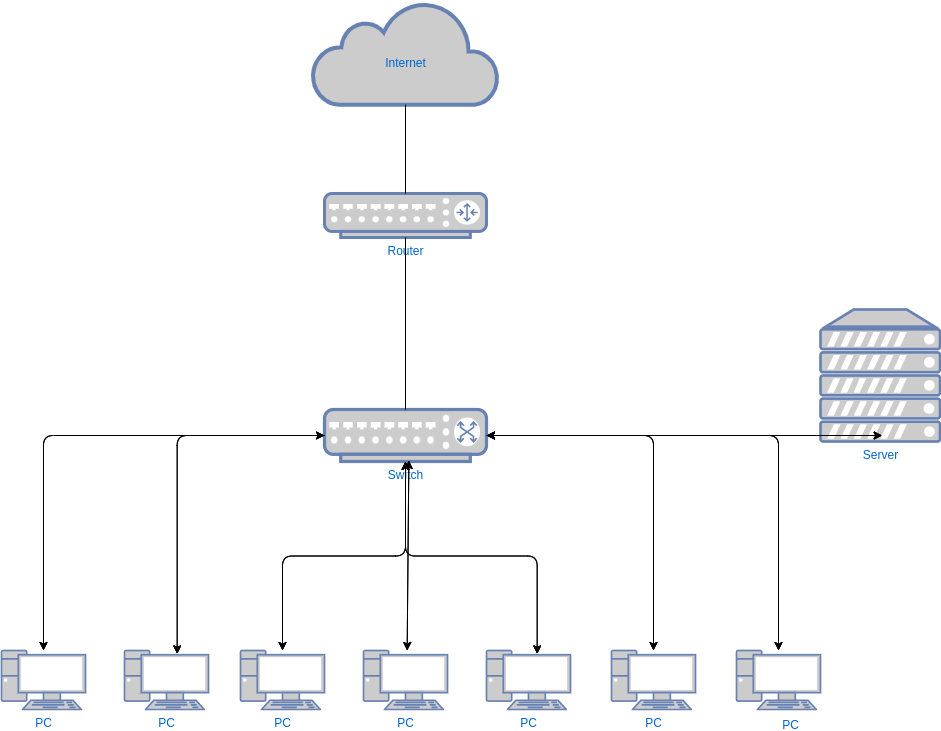
\includegraphics[height=0.6\textwidth]{imagenes/red/diagrama.png}
				\caption{Diagrama de red}
				\label{fig:red local lan}
			\end{figure}
			
				


     \chapter{Servidor Local}\label{ch:servidor}

	\section{¿Que es un Servidor Local}
	
		Definiré a un servidor local como un ordenador que estará permanentemente encendido y conectado a la red LAN. Este ordenador proporcionara una serie de servicios y contenidos sin importar el dispositivo que se utilice. Al no ser consultado directamente no sera necesario tener un monitor y teclado conectado.
		
	\section{Uso del servidor}
	
		El servidor local proporcionara servicio de alojamiento de archivos y Streaming.
		
		\begin{itemize}
			
			\item \textbf{Servidor de archivos:} Permite alojar, sincroniza y compartir archivos con otros
			usuarios y dispositivos que se encuentren en la misma red. Al almacenarse localmente permitirá tener el control total de los datos.
			
			\item \textbf{Servidor Streaming:} gestiona el contenido multimedia (música, películas, series,
			documentales, etc), otorgando la posibilidad de reproducirlo en cualquier dispositivos que se encuentren en la misma red.
			
		\end{itemize}
	
	
	\section{Sistema Operativo}
				
			Por las características propias de Debian no necesitare buscar un sistema operativo orientado a 	servidores, dado que me permitirá crear un potente servidor, al poseer estabilidad/escalabilidad y buenos repositorios.\par
		
	\section{Instalación del Sistema Operativo}\label{install}
			
		Una vez que comience el proceso de instalación, seguiré una serie de pasos que me permitirán instalar y configurar el sistema operativo :
		
		\begin{itemize}
			
			\item \textbf{Graphical Install}
			
			\item \textbf{Localización:} Seleccionar el idioma de instalación que será el idioma utilizado por el sistema. (Por motivos de compatibilidad, se recomienda seleccionar English) Después indicar la localización geográfica del servidor.
			
			\item \textbf{Configure Locale:} Seleccionar “United Estates” para evitar conflictos de compatibilidad.
			
			\item \textbf{Configuración del teclado:} Seleccionar Spanish o Latin America.
			
			\item \textbf{Conexión a Internet:} Para conectarse a Internet se necesita la asignación de una dirección IP a la interfaz de red. La dirección IP y los demás parámetros de la red pueden obtenerse de forma automática a partir de un servidor DHCP o se pueden configurar manualmente.
			
			\item \textbf{Nombre del sistema:} Nombre con el que se conocerá al sistema en la red.
			
			\item \textbf{Cuentas de usuario y passwords:} El programa instalador solicita la creación y configuración de dos cuentas de usuario del sistema o logins. La primera es la cuenta de root y la segunda es una cuenta de usuario ‘normal’, con permisos limitados.
			
			\item \textbf{Reloj del sistema y huso horario:} El instalador intentará sincronizar el reloj del sistema con uno de los servidores que establecen la hora oficial en el Internet.
			
			\item \textbf{Particionado:} Por fines prácticos creare un LVM y seleccionare el método guiado para usar todo el disco. Luego Gestionare el GV de la siguiente manera:
			
			GNU/Linux tiene un nivel de personalización muy amplio, es por ello, que seguramente no todos verán necesario lo que realizare, así como quizás haya alguien que piense que hay muchos otros directorios más susceptibles que no se mencionan y deben alojarse en un (LV).
			
			La gestión de volúmenes consistirá en organizar la raíz del sistema en varios volúmenes. Cada uno de estos pueden tener un objetivo y/o un tipo de sistema de archivos distinto y específico. 
			
			A continuación mencionare los directorios que tendrán su propio (LV), dado el uso que le
			daré al servidor.	
			
			\vspace{0.3cm}
			
			\begin{itemize}
				
				\item \textbf{Directorio /var:} En este directorio se encontraran todo tipo de archivos, de los cuales se espera que en una ejecución normal del sistema estén cambiando continuamente. Estos podrían ser “logs, bases de datos, spool, cachés, e-mail, etc”. \par
									
				\item \textbf{Directorio /tmp:} En este directorio es donde las aplicaciones almacenarán archivos temporales. Tiene la particularidad de que siempre será borrado tras un reinicio del sistema.\par
				
				\item \textbf{Directorio /usr:} Es con frecuencia grande, debido a que todos los programas están instalados aquí. 
				
				\item \textbf{Directorio /srv:}	Sirve para almacenar archivos y directorios relativos a servidores.	
				
				\item \textbf{/var/lib/docker} Los volúmenes se almacenan en /var/lib/docker/volumes/. Docker almacena los datos dentro de este directorio. 
				
				\item \textbf{Directorio /home:} Es donde se crean los directorios de los usuarios normales.
				
				\item \textbf{Directorio /opt:} En este directorio se instalan algunos programas de terceros, además es el directorio donde suelo guardar ejecutables.
				
			\end{itemize}
			
			\item \textbf{Instalación del sistema base:} En este paso el instalador comenzará la instalación de los paquetes de aplicaciones necesarios para crear un sistema base. Este proceso puede tardar algún tiempo.
			
			\item \textbf{Configuración del gestor de paquetes apt:} Seleccionar el repositorio geográficamente más cercano al equipo que se está instalando. En primer lugar se debe elegir el país y luego escoger el mirror más próximo.
			
			\item \textbf{Concurso de popularidad:} La comunidad Debian mantiene un concurso de popularidad interno, con el fin de obtener estadísticas sobre los sistemas instalados. La instalación de este	paquete implica la instalación de otros paquetes. No se recomienda instalar el paquete de popularidad para que el sistema sea lo más ligero posible.
			
			\item \textbf{Finalizar instalación:} El instalador permite la instalación automática de diversas configuraciones del sistema. Como se busca personalizar totalmente el sistema, se anulará cualquier selección existente. De esta forma se instalará un sistema con un mínimo de funcionalidades.
			
			\item \textbf{Instalación del gestor de arranque grub:} En este punto el sistema ya está casi completamente instalado. Sin embargo, para que el sistema pueda arrancar hay que instalar el gestor de arran	que “grub” en el master boot record (mbr) del disco.
			Una vez instalado el grub se debe seleccionar continuar, y el equipo se reiniciara automática mente para el primer login.
		
		\end{itemize}
	
	\section{LVM}
	
		\subsection{¿Que es LVM?}
		
			LVM es una capa de abstracción entre un dispositivo de almacenamiento y un sistema de ficheros. Las ventajas que tienen son múltiples, pero la inicial y por la cual lo uso, es por la flexibilidad frente al particionado tradicional. Con LVM las limitaciones en el redimencionado y particionado desaparecen. Se puede aumentar el tamaño  de los volúmenes lógicos independientemente de que no haya espacio libre contiguo.
				
				\begin{itemize}
					
					\item \textbf{Volumen físico o Physical Volume (PV):} Un volumen físico es un dispositivo de bloque que se le entregará al LVM para que este lo gestione.
					
					\item \textbf{Grupo de volúmenes o Volume Group (VG):} Para poder usar el espacio de almacenamiento de un PV, éste debe pertenecer a un Grupo de volúmenes. Un VG es una especie de disco duro virtual compuesto de uno o más PVs. 
					
					\item \textbf{Volumen Lógico o Logical Volume (LV):} Los volúmenes lógicos son dispositivos en los cuales se crea sistemas de archivos. Por seguir con la analogía del \textit{«disco duro virtual»} que es el VG, los LVs serían las particiones. 
					
				\end{itemize}
			
	
		\subsection{Gestión volúmenes lógicos}
		
			Los volúmenes lógicos son donde todos los datos se almacenan en un LVM. Para crear los nuevos volúmenes lógicos, utilizare los siguiente comandos.

			
			\begin{lstlisting}[language=Bash, caption=Creación de (LV)]
				
			lvcreate -L 10G -n home ema
			lvcreate -L 10G -n docker ema
			lvcreate -L 100G -n srv ema
			lvcreate -L 5G -n opt ema
			lvcreate -L 1G -n tmp ema
			lvcreate -L 15G -n usr ema
			lvcreate -L 1G -n var-tmp ema
			lvcreate -L 1G -n var-log ema
			lvcreate -L 2G -n swap ema
								
			\end{lstlisting}
		
			La sintaxis básica para crear volúmenes lógicos es:
			
			lvcreate \textbf{-L} \textit{«tamaño»}\textbf{G} \textbf{-n} \textit{«nombre del volumen»} \textit{«nombre del grupo»}
			
			\begin{itemize}
				
				\item \textbf{-L} Tamaño en GB o MB.
				\item \textbf{-n} Nombre que tendrá el (LV) Nombre del VG con el que se trabajara.
			 
			\end{itemize}
			
		
			Luego de que los (LVs) estén disponibles, les creare un sistema de archivo:
			
			\begin{lstlisting}[language=Bash, caption=Crear Sistema de Archivo]
						
			mkfs.ext4 /dev/mapper/ema-var--log
			mkfs.ext4 /dev/mapper/ema-var--tmp
			mkfs.ext4 /dev/mapper/ema-tmp
			mkfs.ext4 /dev/mapper/ema-opt
			mkfs.ext4 /dev/mapper/ema-home
			mkfs.ext4 /dev/mapper/ema-docker
			mkfs.ext4 /dev/mapper/ema-usr
			mkfs.ext4 /dev/mapper/ema-srv
			mkswap /dev/mapper/ema-swap
			
			\end{lstlisting}
			
			\vspace{0.3cm}
			
			Una vez creados los sistemas de archivo es hora montar los (LVs) y mover el contenido de los directorios al (LV) correspondiente.
			
			\begin{lstlisting}[language=Bash, caption=Crear directorios y montar los (LVs)]
				
			mv /mnt
			
			mkdir {var-log,opt,home,usr,srv}
			
			mount /dev/mapper/ema-var--log var-log
			mount /dev/mapper/ema-opt opt
			mount /dev/mapper/ema-home home
			mount /dev/mapper/ema-usr usr
			mount /dev/mapper/ema-srv srv
			
			\end{lstlisting}
			
			\vspace{0.3cm}
			
			Mover todo el contenido de los directorios a su	 (LV) correspondiente.
			
			\begin{lstlisting}[language=Bash, caption=Mover directorios]
			
			#Mover el contenido de los directorios
			mv -f var/log/* var-log
			mv opt/* opt
			mv -f home/* home
			mv usr/* usr
			mv srv/* srv
			#Eliminar archivos temporales
			rm -rf var/tmp/*
			rm -rf tmp/*
			
			\end{lstlisting}
		
		
		\section{fstab}
			
			El archivo /etc/fstab es el archivo de configuraciones que une dispositivos con punto de montaje. Le indica al sistema cómo montar cada dispositivo y qué configuración utilizar.\par
			
			Tabla de configuración del archivo fstab: 
			
			\begin{lstlisting}[language=Bash, caption=fstab]
					
			# <file system> <mount point> <type> <options> <dump> <pass>
			
			\end{lstlisting}
			
			\begin{itemize}
				 
				\item \textbf{file system:} Esta primera columna guarda el dispositivo a montar. 
				
				\item \textbf{mount point:}	Esta opción permite definir el directorio que se va a asociar con el (LV) definido en la primera columna. 
				
				\item \textbf{Tipo:} Este campo se refiere al tipo de filesystem, por ejemplo, ext4, xfs, entre otros.
				
				\item \textbf{Opciones:} Hace referencia a las opciones de montaje. Deben ir separadas por comas. 
				
				Algunas de las opciones que se pueden usar son:
				
				\begin{itemize}
				 	
					\item \textbf{auto:} para que la partición se monte al arrancar.
					
					\item \textbf{noauto:} opción que impide que la partición se monte durante el arranque.
					
					\item \textbf{user:} los usuarios tienen permitido montar la partición.
					
					\item \textbf{nouser:} solo el usuario root tiene permitido realizar el montaje de la partición.
					
					\item \textbf{ro:} partición que solo permite la lectura.
					
					\item \textbf{rw:} opción que permite la lectura escritura.
					
					\item \textbf{exec:} es posible ejecutar los binarios pertenecientes a esa partición.
					
					\item \textbf{async:} esta opción permite que el sistema continúe trabajando luego de una petición de escritura del equipo, aunque no haya recibido la confirmación.
				
					\item \textbf{suid:} esta opción permite las operaciones con los bits suid y sgid. Es utilizado para permitir a los usuarios diferentes del root, ejecutar binarios con ciertos privilegios otorgados temporalmente para que realicen una labor determinada.
					
					\item \textbf{nosui:} se encarga de impedir el funcionamiento de los bits suid y sgid.
					
					\item \textbf{noatime:} esta opción no actualiza el nodo-i de los ficheros con el tiempo de acceso. Además, permite aumentar las prestaciones del sistema, debido a que accede menos al disco.
					
					\item \textbf{nodiratime:} con esta opción se impide la actualización del nodo-i de los directorios con el tiempo de acceso. Al igual que la opción noatime, también puede aumentar las prestaciones del sistema.
				
					\item \textbf{defaults:} establece que las opciones sean asignadas por defecto gracias al sistema operativo. Estas opciones predeterminadas son  rw, suid, dev, exec, auto, nouser y async.
				
				\end{itemize}
	
				\item \textbf{Soporte a Dump:} Este campo es requerido por algunas soluciones de backup. Además, determina la frecuencia con la que debe realizarse la copia de seguridad.
				
				\item \textbf{Chequeo automático:} Es el campo encargado de especificar si el sistema de ficheros debe ser revisado durante el arranque, si el formato es correcto, entre otros. Normalmente ese campo se deshabilita para todas las particiones, a excepción del /.
				
			\end{itemize}
		
			\subsection{Configurar fstab}
			
				Es necesario que defina que los (LVs) se monten automáticamente cuando se está iniciando el sistema operativo. La forma correcta para resolver este problema es modificando el archivo fstab.
				
				Finalizada la configuración mi archivo fstab quedara de la siguiente manera:

				\vspace{0.3cm}
									
				\inputminted{bash}{documentos/fstab/fstab}
	
	\section{Controlar cambios en el sistema}
		
		Por cuestiones de seguridad tomo como buena practica generar HASH de los archivos que se encuentran en algunos directorios que considero importante, por si en algún momento tengo la duda de que se generaron cambios en el sistema, poder realizar las comparaciones de HASH.
	
		\clearpage
		
		\subsection{Generar Hash}
			
			md5sum es un algoritmo de reducción criptográfico de 128-bits desarrollado por MIT. Se utiliza con frecuencia como herramienta para validar un archivo.
			
			\inputminted{bash}{documentos/seguridad/generarHash.sh}
					
		
		\subsection{Comparar Hash}
			
			Si por alguna razon necesito validar la integridad de los archivos del sistema, utilizo el siguiente script en bash.
		
			\inputminted{bash}{documentos/seguridad/compararHash.sh}
			
	\section{Configuración de red}
	
		\subsection{Asignar una IP estática}
			
			El servidor tendrá una dirección IP estática, la cual se la asignare editando el archivo \textit{"interfaces"}.\par
			
			\begin{lstlisting}[language=Bash, caption=Interfaces]		
				nvim /etc/network/interfaces	
			\end{lstlisting}
			
			A continuación presento el contenido del archivo /etc/network/interfaces con una configuración de IP estática:
			
			\begin{lstlisting}[language=Bash, caption=Configuración de IP estática]	
				# This file describes the network interfaces available on your system
				# and how to activate them. For more information, see interfaces(5).	
				source /etc/network/interfaces.d/*
				# The loopback network interface
				auto lo
				iface lo inet loopback	
				# Interfaz de red enp2s0
				auto enp2s0
				allow-hotplug enp2s0
				iface enp2s0 inet static
					address   192.168.1.222
					netmask   255.255.255.0
					network   192.168.1.0
					broadcast 192.168.1.255
					gateway   192.168.1.1
			\end{lstlisting}
			
			\begin{itemize}
				
				\item \textbf{iface enp2s0 inet static:} define el nombre lógico de la interfaz de red enp2s0,
				la \textit{address\_family} que es \textbf{inet} y el método de configuración de la interfaz que es \textbf{static}.
				
				\item \textbf{address:} define la IP que tendrá el servidor.
			
				\item \textbf{netmask:} define la máscara de subred.
			
				\item \textbf{network:} define la dirección de red.
			
				\item \textbf{broadcast:} define la IP de difusión (broadcast).
			
				\item \textbf{gateway:} define la IP de la puerta de enlace (gateway).
			
			\end{itemize}
						
			Una vez finalizada la edición del archivo reiniciare el servicio de red para aplicar los cambios. \par
			
									
			\begin{lstlisting}[language=Bash, caption=Reiniciar servicio de RED]			
				systemctl restart networking.service
			\end{lstlisting}
			
		
		\subsection{Servidor DNS}
			
		
			Es necesario que tambien configure los servidores DNS. Para configurarlos editare el archivo /etc/resolv.conf:\par
	
		
			\begin{lstlisting}[language=Bash, caption=Editar archivo resolv]		
				nvim /etc/resolv.conf
			\end{lstlisting}
		
			
			A continuación presento el contenido del archivo /etc/resolv.conf con dos servidores DNS:

		
			\begin{lstlisting}[language=Bash, caption=Servidores DNS]	
			# Dynamic resolv.conf(5) file for glibc resolver(3) generated by resolvconf(8)
			#     DO NOT EDIT THIS FILE BY HAND -- YOUR CHANGES WILL BE OVERWRITTEN	
			nameserver 1.1.1.1    
			nameserver 8.8.8.8
			\end{lstlisting}
		

			\begin{itemize}
				
				\item \textbf{1.1.1.1:} Es un DNS público operado por Cloudflare que ofrece una forma rápida y privada de navegar por Internet. A diferencia de la mayoría de los servidores de DNS, 1.1.1.1 no vende los datos de los usuarios a los anunciantes.

				\item \textbf{8.8.8.8:} Como una forma de hacer más rápida la web Google tiene, Google Public DNS. Que es una forma de navegar fuera de los límites del proveedor de servicios de internet.

			\end{itemize}

				
	\section{Firewall}
		
		\subsection{¿Que es iptables?}
		
			Iptables es una herramienta de filtrado de paquetes en Linux. Se encarga de analizar cada uno de los paquetes del tráfico de red que entra en una máquina y decidir, en función de un conjunto de reglas, qué hacer con ese paquete.
			
			Gracias a la capacidad de analizar el tráfico y ver las características del paquete, se puede implementar un cortafuegos que controle qué paquetes puede llegar al equipo.
			
			\subsubsection{Características de iptables:}
			
				\begin{itemize}
					\item Es el sucesor de ipfwadm e ipchains, un software previo que existía en sistemas Linux.
				
					\item Se encuentra disponible desde la rama 2.4 del kernel de Linux, que se lanzó el año 2001.
				
					\item Está desarrollado por el proyecto netfilter. Este mismo proyecto ha desarrollado también el sucesor de iptables, que se denomina nftables, aunque en la actualidad todavía está mucho más extendido el uso de iptables que el de nftables.
					
				\end{itemize}		
			
			\subsection{Reglas iptables}
			
				El siguiente script en bash me permitirá configurar el el firewall de linux.
			
				\inputminted{bash}{documentos/firewall/firewall.sh}
	
			
	\section{Servidor Docker}
	
		\subsection{¿Que es Docker?}
		
			Docker es una plataforma de contenerización de código abierto. Permite a los desarrolladores empaquetar aplicaciones en contenedores. Los contenedores combinan el código fuente de la aplicación con las bibliotecas del sistema operativo y las dependencias necesarias para ejecutar el código en cualquier entorno. Los contenedores simplifican la entrega de aplicaciones distribuidas.\par
			
			Docker es esencialmente un kit de herramientas que permite a los desarrolladores crear, implementar, ejecutar, actualizar y detener contenedores utilizando comandos a través de una única API.
			
		\subsection{Funcionamiento de los contenedores?}
			
			Los contenedores son posibles gracias al aislamiento de procesos y a las capacidades de virtualización integradas en el kernel de Linux. Estas funcionan como grupos de control (Cgroups) para asignar recursos entre procesos, y espacios de nombres para restringir un acceso de procesos o visibilidad a otros recursos o áreas del sistema.\par
			
			Como resultado, los contenedores ofrecen toda la funcionalidad y beneficios de las máquinas virtuales, incluyendo aislamiento de aplicaciones, escalabilidad y capacidad de disposición. Sus ventajas son las siguientes:\par
			
						
			\begin{itemize}
				
				\item \textbf{Ligero:} Los contenedores sólo incluyen los procesos y dependencias del sistema operativo necesarias para ejecutar el código.
				
				\item \textbf{Mejor manejo de los recursos:} Con contenedores se puede ejecutar varias veces las mismas copias de una aplicación en el mismo hardware.
				
				\item \textbf{Mayor productividad de los desarrolladores:} En comparación con las VM, los contenedores son más rápidos y fáciles de implementar, suministrar y reiniciar.
			
			\end{itemize}
			
		\subsection{Características}
		
			\vspace{0.3cm}
				
			\begin{itemize}
					
				\item \textbf{Portabilidad:} Los contenedores LXC suelen hacer referencia a 		configuraciones especificas de la máquina, mientras que los contenedores Docker se ejecutan sin modificaciones en cualquier entorno de escritorios, centro de datos y nube.
				
				\item \textbf{Ligeros:} Con los contenedores Docker solo se puede ejecutar un proceso en cada contenedor. Esto permite crear una aplicación que puede continuar ejecutándose mientras una de sus partes se desactiva.
									
				\item \textbf{Creación automática de contenedores:} Docker puede crear automáticamente un contenedor basado en el código de origen de la aplicación.
				
				\item \textbf{Control de versiones:} Docker puede rastrear versiones de una imagen de contenedor, retroceder a versiones anteriores y rastrear quién creó una versión. 
			
				\item \textbf{Reutilizar contenedores:} Los contenedores existentes se pueden utilizar como imágenes base, esencialmente como plantillas para crear nuevos contenedores.
				
				\item \textbf{Repositorio de contenedores:} Los desarrolladores pueden acceder a un registro de código abierto que contiene miles de contenedores aportados por los usuarios.
			
			\end{itemize}
			
		\subsection{Herramientas de Docker}
			
			\vspace{0.3cm}
			
			\begin{itemize}
					
				\item \textbf{DockerFile:} Cada contenedor Docker se inicia con un archivo de texto simple que contiene instrucciones para crear la imagen del contenedor Docker. El DockerFile es una lista de instrucciones de interfaz de línea de comandos que Docker Engine ejecutará para ensamblar la imagen.
				
				\item \textbf{Imágenes Docker:} Las imágenes Docker contienen el código de origen de la aplicación, herramientas, bibliotecas y dependencias que el código de la aplicación debe ejecutar como contenedor.\par
				
				Las imágenes Docker son archivos de sólo lectura.
				
				\item \textbf{Contenedores Docker:} Los contenedores Docker son las instancias activas en ejecución de imágenes Docker.\par
				 
				Los contenedores son contenido en vivo, efímero y ejecutable. Se pueden interactuar con ellos utilizando comandos Docker.
				
				\item \textbf{Docker Hub:} Es el repositorio público de imágenes Docker. Las imágenes de contenedor provienen de proveedores de software comercial, proyectos de código abierto y desarrolladores individuales. Ademas de las imágenes que han sido producidas por Docker, Inc.\par
				
				\item \textbf{Daemon Docker:} El daemon Docker es un servicio que se ejecuta en el sistema operativo. Este servicio crea y gestiona las imágenes Docker.
				

			\end{itemize}
		
		
		\subsection{Instalación Docker}
			
			\vspace{0.1cm}
			
			Antes de comenzar con la instalación es necesario que se instalen unas herramientas:
					
			\begin{itemize}
				
				\item\textbf{apt-transport-https:} permite que el administrador de paquetes transfiera datos a través de https.
				
				\item\textbf{ca-certificates:} permite que el navegador web y el sistema verifiquen los certificados de seguridad.
				
				\item\textbf{curl:} transfiere datos.
				
				\item \textbf{software-properties-common:} agrega scripts para administrar el software.
				
			\end{itemize}	
				
				
			\begin{lstlisting}[language=Bash, caption=Paquetes necesarios]
	#actualizar lista de paquetes
	apt update
	#instalar herramientas
	apt install curl apt-transport-https ca-certificates software-properties-common
	
			\end{lstlisting}
			
			\textbf{Clave GPG:}\par
			
			\begin{lstlisting}[language=Bash, caption=Clave GPG]
	#crear directorio
	mkdir -p /etc/apt/keyrings
	#descargar key
	curl -fsSL https://download.docker.com/linux/debian/gpg | gpg --dearmor -o /etc/apt/keyrings/docker.gpg
			\end{lstlisting}
		
			\textbf{Agrega el repositorio:}
	
			\begin{lstlisting}[language=Bash, caption=Repositorio]

	#agregar repositorio
	echo "deb [arch=$(dpkg --print-architecture) signed-by=/etc/apt/keyrings/docker.gpg] https://download.docker.com/linux/debian $(lsb_release -cs) stable" | sudo tee /etc/apt/sources.list.d/docker.list > /dev/null
			\end{lstlisting}
	
			\textbf{Instalar Docker Engine.}\par
	
	
			\begin{lstlisting}[language=Bash,caption=docker]
	#actualizar lista de paquetes
	apt update
	#instalar docker
	apt install docker-ce docker-ce-cli containerd.io docker-compose-plugins
			\end{lstlisting}


			Para verificar que docker se esta ejecutando correctamente ejecutare el contenedor de Hello-World, el cual da una bienvenida.
	
			\begin{lstlisting}[language=Bash,caption=Hello-World]
	#descargar y ejecutar contenedor de bienvenida
	docker run hello-world
			\end{lstlisting}
		
		\subsection{¿Que es Docker Compose?}
		
			Docker Compose es una herramienta que permite simplificar el uso de Docker a partir de un archivo YAML. De esta manera es mas sencillo crear contendores, conectarlos, habilitar puertos, volúmenes, etc.\par 
		
		\subsection{Instalación Docker Compose}
			
			\vspace{0.2cm}
			
			Hay varias versiones de Docker Compose, aunque siempre es preferible la versión estable.

									
			\begin{lstlisting}[language=Bash,caption=Docker Compose]
	#descargar binario de docker-compose	
	curl -L "https://github.com/docker/compose/releases/download/1.26.0/docker-compose-$(uname -s)-$(uname -m)" -o /usr/local/bin/docker-compose
	#cambiar permisos
	chmod +x /usr/local/bin/docker-compose
	#controlar la version de docker-compose
	docker-compose --version
			\end{lstlisting}
				
				
	\section{Contenedor NextCloud}
		
		\subsection{¿Que es Nextcloud?}
		
			Nextcloud es un servidor para el intercambio de archivos que permite almacenar contenido personal (documentos e imágenes, videos, etc) en una ubicación centralizada. Al ser sus funciones de código abierto, ofrece una gran versatilidad, seguridad y cumplimiento a las normas de privacidad. También permite aplicar diferentes políticas a los datos, como cifrado, administración de usuarios y auditoría.\par
		
	
			\subsection{Características:}
		
				\begin{itemize}
					
					\item Los archivos Nextcloud son almacenados en estructuras de directorio convencionales y se
					pueden acceder vía WebDAV.
					
					\item Los archivos son cifrados en la transmisión y opcionalmente durante el almacenamiento.
					
					\item Los usuarios pueden manejar calendarios CalDAV, contactos CardDAV, tareas programadas y
					reproducir contenido multimedia Ampache.
					
					\item Permite la administración de usuarios y grupos de usuarios, vía OpenID o LDAP y definir per-
					misos de acceso.
					
					\item Posibilidad de añadir aplicaciones de un solo clic y conexiones con Dropbox, Google Drive y
					Amazon S3.
					
					\item Disponibilidad de acceso a diferentes bases de datos, mediante SQLite, MariaDB, MySQL,
					Oracle Database, y PostgreSQL
					
					\item Cuenta con aplicaciones clientes para Windows, MAC OSX, Linux, Android y IOS.\par
					
					
				\end{itemize}

			\subsection{Requisitos:}
		
				
				Al ejecutarse dentro de un contenedor todas sus dependencias se encuentran resueltas, solo se debera considerar la cantidad de memoria RAM.\par
					
				La documentación de Nextcloud indica que la cantidad de memoria que se necesita para ejecutar un servidor Nextcloud es muy variable, y dependerá de la cantidad de usuarios, aplicaciones, archivos y volumen de actividad del servidor.\par
			
			\subsection{Preparación del área de trabajo}
				
				Mi directorio de trabajo sera \textit{/srv} donde creare un directorio que almacenara toda las configuraciones de Nextcloud, asi como la configuración de la base de datos.
				
				\begin{lstlisting}[language=Bash,caption=Directorio de trabajo NextCloud]
			#cambiar al directorio /srv
			cd /srv
			#crear directorio Nextcloud
			mkdir nextcloud
			#entrar al directorio Nextcloud
			cd nextcloud
				\end{lstlisting}
			
				Dentro del directorio creare un documento llamado \textit{docker-compose.yaml} y dentro de el colocare el siguiente código:
	
				\inputminted{yaml}{documentos/docker/nextcloud/docker-compose.yml}
			
				\subsubsection{Estructura del docker-compose.yml}\label{estructura-docker}
				
					\begin{itemize}
						
						\item \textbf{version:} Un archivo de docker-compose comienza especificando la versión de docker compose que se utilizará.
							
						\item \textbf{services:} Después de la versión viene anidada la sección de \textit{services}. Puede haber tantos servicios como se necesiten, y cada servicio contará con sus propia estructura.
						
						\item \textbf{image:} La configuración \textit{image} establece la imagen a partir de la cual se generará el servicio.
						
						\item \textbf{container\_name:} El nombre que tendra el contenedor cuando se este ejecutando.
						
						\item \textbf{environment:} La configuración environment permite establecer una lista de variables de entorno que estarán disponibles en el servicio.
						
						\item \textbf{volumes:} Con volúmenes se puede compartir partes del sistema operativo con un servicio.
						
						\item \textbf{ports:} Los puertos que se expondrán al exterior y a cual puerto de la máquina se vincularán.
						
						\item \textbf{restart:}	Con restart se especifica la política de reinicio a los servicios.
						
						La opción restart puede tomar varios valores:
					
						\begin{itemize}
							
							\item \textbf{no:} nunca reinicia el contenedor.
							
							\item \textbf{always:} siempre lo reinicia.
							
							\item \textbf{on-failure:} lo reinicia si el contenedor devuelve un estado de error.
							
							\item \textbf{unless-stopped:} lo reinicia en todos los casos excepto cuando se detiene.
						
						\end{itemize}
						
					\end{itemize}
				
			
		\subsection{Crear Contenedor}
		
			Para crear el contenedor de Nextcloud es necesario que se utilice el siguiente comando, el cual descargara las imágenes necesarias y realizara las configuraciones especificadas dentro del archivo YAML.
			
			\begin{lstlisting}[language=bash,caption=Crear Contenedor Docker]		
				
				docker-compose up -d
			\end{lstlisting}	
					
			\subsubsection{Explicación del comando anterior:}\par
			
				\begin{itemize}
				
					\item \textbf{docker-compose:} Define y ejecute aplicaciones de varios contenedores con Docker.
				
					\item \textbf{up:} Crea e inicia el contenedor.
				
					\item \textbf{-d:} Ejecuta contenedores en segundo plano.
				 
				\end{itemize}
			
			En caso que Docker deba descargar las imágenes, este proceso puede demorar varios minutos, dependiendo de la velocidad de la conexión al Internet con la que se cuente.\par
						
			Para visualizar si los contenedores se están ejecutando correctamente Docker permite ver el estado de los contenedores con el siguiente comando:
			
			\begin{lstlisting}[language=bash,caption= Estado de los contenedores]
			
			docker ps -a
			\end{lstlisting}
	
		\subsection{Configuración de NextCloud}	
			
			Una vez que el contenedor de Nextcloud se encuentre corriendo, desde el navegador web terminare de realizar las configuraciones:

			
			\begin{itemize}
				
				\item Crear usuario administrador.
				\item Expecificar el directorio donde se guardan los datos que se almacenen en Nextcloud.
				\item Configurar la base de datos.
				
			\end{itemize}
			
			\begin{figure}[h]
				
				\centering
				
				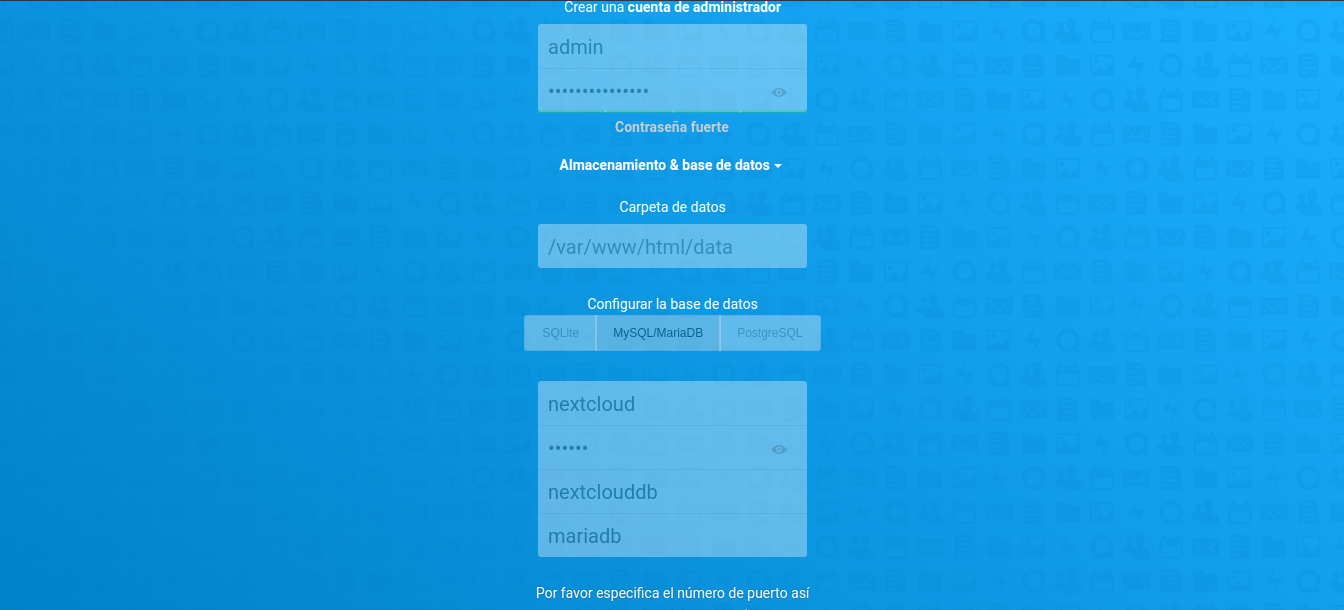
\includegraphics[width=0.9\textwidth]{imagenes/docker/nextcloud/configurarNextcloud.png}
				
				\caption{Configurar Nextcloud}
				
				\label{fig:nextcloud}
				
			\end{figure}
			
			\pagebreak
			
			\begin{tcolorbox}[enhanced,frame style image=blueshade.png,opacityback=0.75,opacitybacktitle=0.25, colback=blue!5!white,colframe=blue!75!black,title=Nextcloud]
				Para acceder a NextCloud en el navegador se debe colocar la dirección IP del servidor Docker y el puerto donde escucha el contenedor. En mi caso seria \href{http://192.168.1.222:8080/}{\color{blue}http://192.168.1.222:8080}
			\end{tcolorbox}
			
			Finalizada la configuración y ya dentro del dashboard me dirigiré al perfil del usuario administrador, donde podre crear los usuarios que tendrán acceso al servicio de Nextcloud.
			
			\begin{figure}[h]
				
				\centering
				
				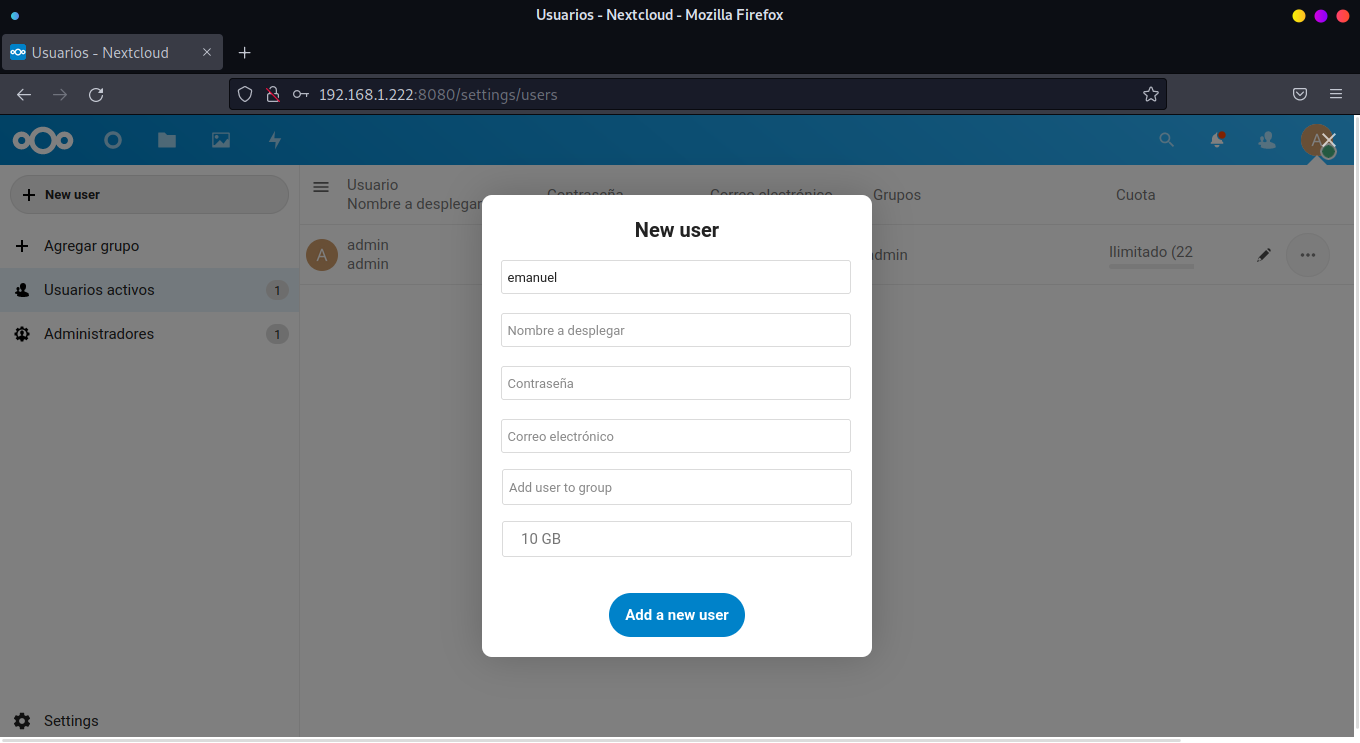
\includegraphics[width=0.9\textwidth]{imagenes/docker/nextcloud/creacionUsuarios.png}
				
				\caption{Creación de Usuarios}
				
				\label{fig:usuarios}
			\end{figure}	
		
		Los alumnos podrán hacer uso de este servicio solamente desde la red lan a través de un navegador web. Donde cada uno accederá con su usuario y contraseña.\par
		
		\subsection{Conclusión}
			
			Con Nextcloud la información se almacena de forma segura en un lugar controlable. NextCloud replicar las capacidades de servicios externos de almacenamiento en la nube, permitiendo compartir contenido entre usuarios de la misma red local.

	\section{Contenedor Emby}
	
		\subsection{¿Que es Emby?}
		
			Emby es un centro de multimedia multiplataforma que permite visualizar contenido desde cualquier tipo de dispositivo via Web, App o DLNA. 
		
			Emby trabaja con el contenido multimedia almacenado en servidor local, esto lo hace ideal dadas las características del Aula Virtual.\par
			
		\subsection{Características de Emby:}
			
			\begin{itemize}
				
				\item El servidor de Emby convierte y envía automáticamente los vídeos a cualquier dispositivo.
				
				\item Cuenta con canales de vídeo en directo.
				
				\item Permite sincronizar librerías con los clientes móviles.
				
				\item La organización está muy cuidada para ser sencilla de ver y entender.
				
				\item Cuenta con controles parentales.
				
				\item Servidor DLNA para reproducir el contenido multimedia.
				
				\item Compatible con Chromecast.
	
			\end{itemize}
		
		\subsection{¿Qué es un centro multimedia?}
		
			Un centro multimedia es una aplicación que gestiona el contenido multimedia (fotografías, musica y vídeos), para que se pueda reproducir en el mismo dispositivo donde esta almacenado o en otros dispositivos, en este caso, conectados a la red LAN.
		
			Emby, cuentas con la aplicación servidor que gestiona el contenido y lo transmite por streaming, y por otro lado la aplicación que recibe el contenido. La cual puede ser el cliente que se encuentra disponible para la plataforma de Windows, Mac, Linux, FreeBSD, dispositivos NAS, Android, iOS, Windows Phone, Android TV, Fire TV, Apple TV, Kodi, Xbox, etc. O  cualquier navegador compatible con HTML5.
		
		\subsection{Preparación del área de trabajo}
			
			Mi directorio de trabajo sera /srv donde creare un directorio que almacenara toda las configuraciones de Emby.\par
			
			\begin{lstlisting}[language=Bash,caption=Directorio de trabajo Emby]
				#cambiar al directorio srv
				cd /srv
				#crear directorio
				mkdir emby
				#cambiar directorio
				cd emby
			\end{lstlisting}
			
			\clearpage
			
			Dentro del directorio creare un documento docker-compose.yaml el cual contendra el siguiente codigo:
								
			\inputminted{yaml}{documentos/docker/emby/docker-compose.yml}
			
			\begin{tcolorbox}[enhanced,attach boxed title to top center={yshift=-3mm,yshifttext=-1mm},
			colback=blue!5!white,colframe=blue!75!black,colbacktitle=red!80!black,title= Estructura del documento,fonttitle=\bfseries, boxed title style={size=small,colframe=red!50!black} ]
			
			\centering
			
				Descripción del código \ref{estructura-docker}
			
			\end{tcolorbox}
			
			\subsection{Crear Contenedor Docker:}\par\vspace{0.2cm}
			
			\begin{lstlisting}[language=bash,caption=Crear contenedor Docker]
	
				docker-compose up -d
			\end{lstlisting}	
			
			\subsubsection{Explicación del comando anterior:}\par
			
			\begin{itemize}
				
				\item \textbf{docker-compose:} Define y ejecute aplicaciones de varios contenedores con Docker.
				
				\item \textbf{up:} Crea e inicia el contenedor.
				
				\item \textbf{-d:} Ejecuta contenedores en segundo plano.
				
			\end{itemize}
			
			Este proceso puede demorar varios minutos, dependiendo de la velocidad de la conexión al Internet con la que se cuente. Una vez finalizada la descarga de la imágene se ejecutara el contenedor.\par
	
		\subsection{Configuración Emby}
					
			Una vez que el contenedor se encuentra en ejecución me dirigiré al navegador web para terminar de realizar las configuraciones. Al igual que en NextCloud, para acceder al servicio de Emby solo se debe colocar en el navegador web la dirección IP del servidor Docker y el puerto donde escucha. En mi caso seria \href{http://192.168.1.222:8096/}{\color{blue}http://192.168.1.222:8096}
			
			\begin{itemize}
				
				\item \textbf{Idioma:} Seleccionar el lenguaje de la Interfaz Emby.
				
				\item \textbf{Crear usuario y contraseña:} Creación del usuario para acceder a la interfaz web de Emby.
				
				\item \textbf{Agregar Contenido Multimedia:} Seleccionar los directorios donde se encuentran todo el contenido multimedia que se compartirá con la red lan.
				
				\item \textbf{Lenguaje de las Bibliotecas:} Seleccionar el Lenguaje con el que se mostrara la información del contenido multimedia en la plataforma web.
				
				\item \textbf{Términos y Condiciones:} Aceptar los términos y condiciones de Emby.
				
				\item \textbf{Final de Configuración:} Ahora Emby se encargara de realizar las demás configuraciones, mientras ofrece los clientes de todas las plataformas soportadas.
				
				\item \textbf{Login:} Ingresar al sistema web.
				
			\end{itemize}
		
			\subsubsection{Panel de control de Emby}
			
				\begin{figure}[h]
					
					\centering
					
					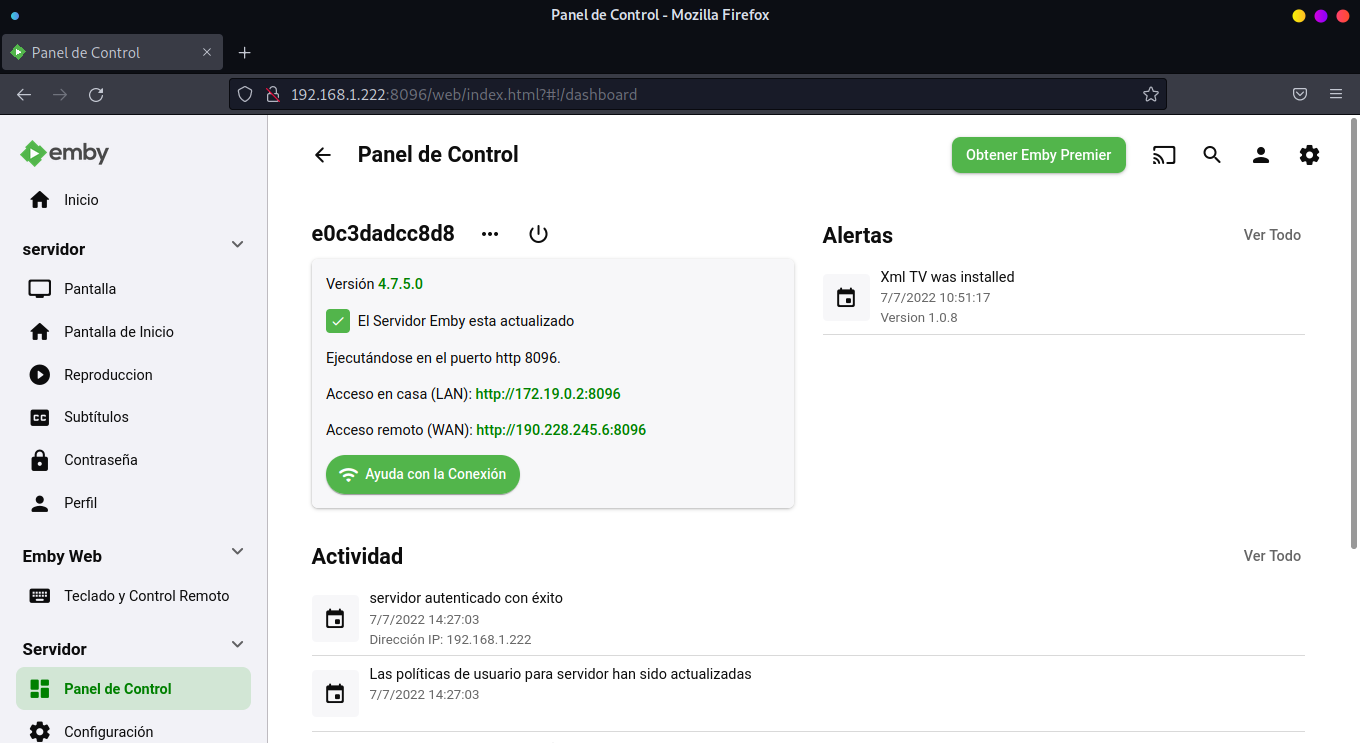
\includegraphics[width=0.9\textwidth]{imagenes/docker/emby/emby-dashboard.png}
					
					\caption{Dashboard}
					
					\label{fig:dashboard}
					
				\end{figure}
					
		\subsection{Conclusión}
		
			Uno de los problemas que tenemos en el Aula virtual es la velocidad de conexión al Internet (2MB). Lo que dificulta en gran manera la reproducción de Vídeos Tutoriales o contenido multimedia recomendado por los docentes.\par
			
			Ahora se descarga el contenido multimedia y se almacena de forma segura en un lugar controlable dentro del Servidor Local y con Emby por medio de streaming se comparte con toda la red lan.\par
	 %problemas con los espacion. muchos espacios en blanco y saltos de linea
    
    \chapter{Conclusión}\label{ch:Conclusión}

En este plan de migración se han considerado los programas privativos que se utilizan actualmente y sus respectivas alternativas en software libre. Según los resultados obtenidos a partir de la investigación y búsqueda de alternativas libres, se puede concluir que la migración a software libre es factible si los alumnos están de acuerdo.\par

Cabe destacar que uno de los factores más importantes en la búsqueda de información fue la comunidad de software libre, la cual está conformada en su mayoría por usuarios finales. Estos mismos usuarios sirvieron de guía y ayuda para enfocarse en la elaboración de una estrategia que permita afrontar el problema propuesto. Con la ayuda de sus recomendaciones, se llegó a la conclusión de que se requiere una capacitación y formación adecuada para trabajar en el nuevo entorno de trabajo. En el caso de la persona responsable de la migración e implementación, asumirá el tiempo asociado al entrenamiento, capacitación, formación y soporte a los alumnos.\par

Como trabajo futuro, se propone la ampliación de este proyecto, la generación de una política de seguridad, una administración centralizada y una planificación más detallada del proceso de migración.

Como señala Stallman, es importante que en escuelas y universidades se utilice software libre, ya que estas instituciones educativas están decidiendo el futuro de la sociedad. Por lo tanto, no se debe aceptar que en un espacio perteneciente a la universidad se utilice y enseñe a utilizar software privativo, sabiendo que el deber de una universidad es la creación y difusión del conocimiento. Los alumnos, como parte de ella, también deben defender la libertad de las personas para compartir el conocimiento y el software.	

	
	
	\vspace{0.3cm}
	
	\begin{quote}
		
		\begin{flushright}
			
		{\small	«Las escuelas deben enseñar a sus alumnos a ser ciudadanos de una sociedad fuerte, capaz, independiente y libre».\par
		
		The Free Software Foundation.}
		
	\end{flushright}

		
	\end{quote}


    
    \backmatter
    
    \nocite{*}
    
    \bibliographystyle{plain}
    
    \bibliography{cuerpo/bibliografias/bd-bibliografias.bib}
       
\end{document}


